% P1 (2026-11-24): derived from appendix_e4_all12_figures_layout_v2_20261123.tex (unchanged).
% Changed: header, section title, intro paragraph, and missing-figure fallback text only.
% All \includegraphics paths, captions and labels are byte-identical to layout V2.
\section{全部12张DLPFC切片的空间分布图件}
\label{sec:cc-e4-appendix-v1}
本附录列出全部12张DLPFC切片的空间聚类图、标记基因表达图与参考层--聚类交叉计数图，作为第\ref{subsec:cc-res-maps-p1}节的完整补充。所有图件均使用随机种子22911、参考类别数条件下A、B两种15维组合的原始预测；聚类编号未依据参考标签重排。12张切片来自3名供体，不构成12个独立的生物学重复。图件由原始计数与预测直接绘制，未作任何重绘或生成式处理。

\subsection{DLPFC切片151507}
\IfFileExists{E4_SOURCE_FIGURES_20261122_RELEASE/figures_pdf/151507/151507_reference_A_B_spatial.pdf}{%
\par\noindent\begin{minipage}{\linewidth}
\centering
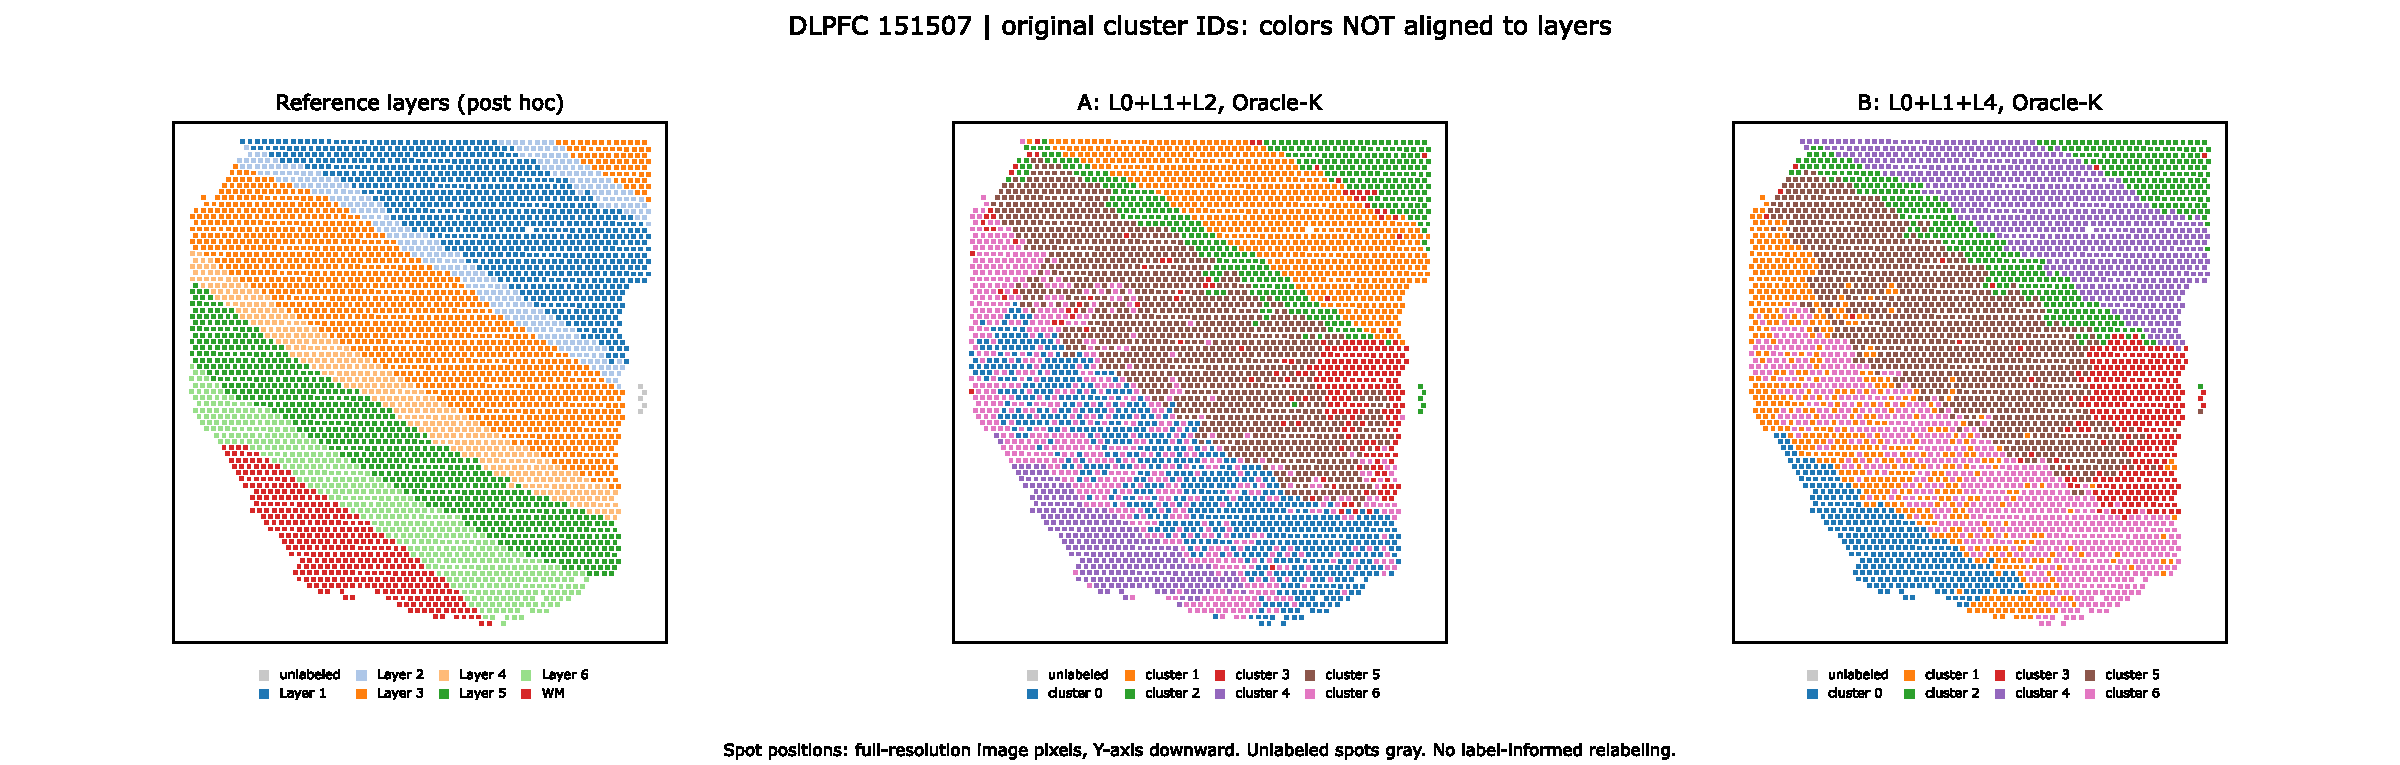
\includegraphics[width=0.97\linewidth,height=0.72\textheight,keepaspectratio]{E4_SOURCE_FIGURES_20261122_RELEASE/figures_pdf/151507/151507_reference_A_B_spatial.pdf}
\captionof{figure}{DLPFC切片151507：参考层与A/B原始聚类三联图（原始E4图件转换的矢量PDF；聚类编号未根据参考标签重排）。}
\label{fig:cc-e4-app-151507-map}
\end{minipage}\par\medskip
}{%
\par\noindent\emph{[编译提示：未找到该图件的PDF，请检查相对路径。]}\par
}
\IfFileExists{E4_SOURCE_FIGURES_20261122_RELEASE/figures_pdf/151507/151507_MOBP_PCP4_SNAP25_expression.pdf}{%
\par\noindent\begin{minipage}{\linewidth}
\centering
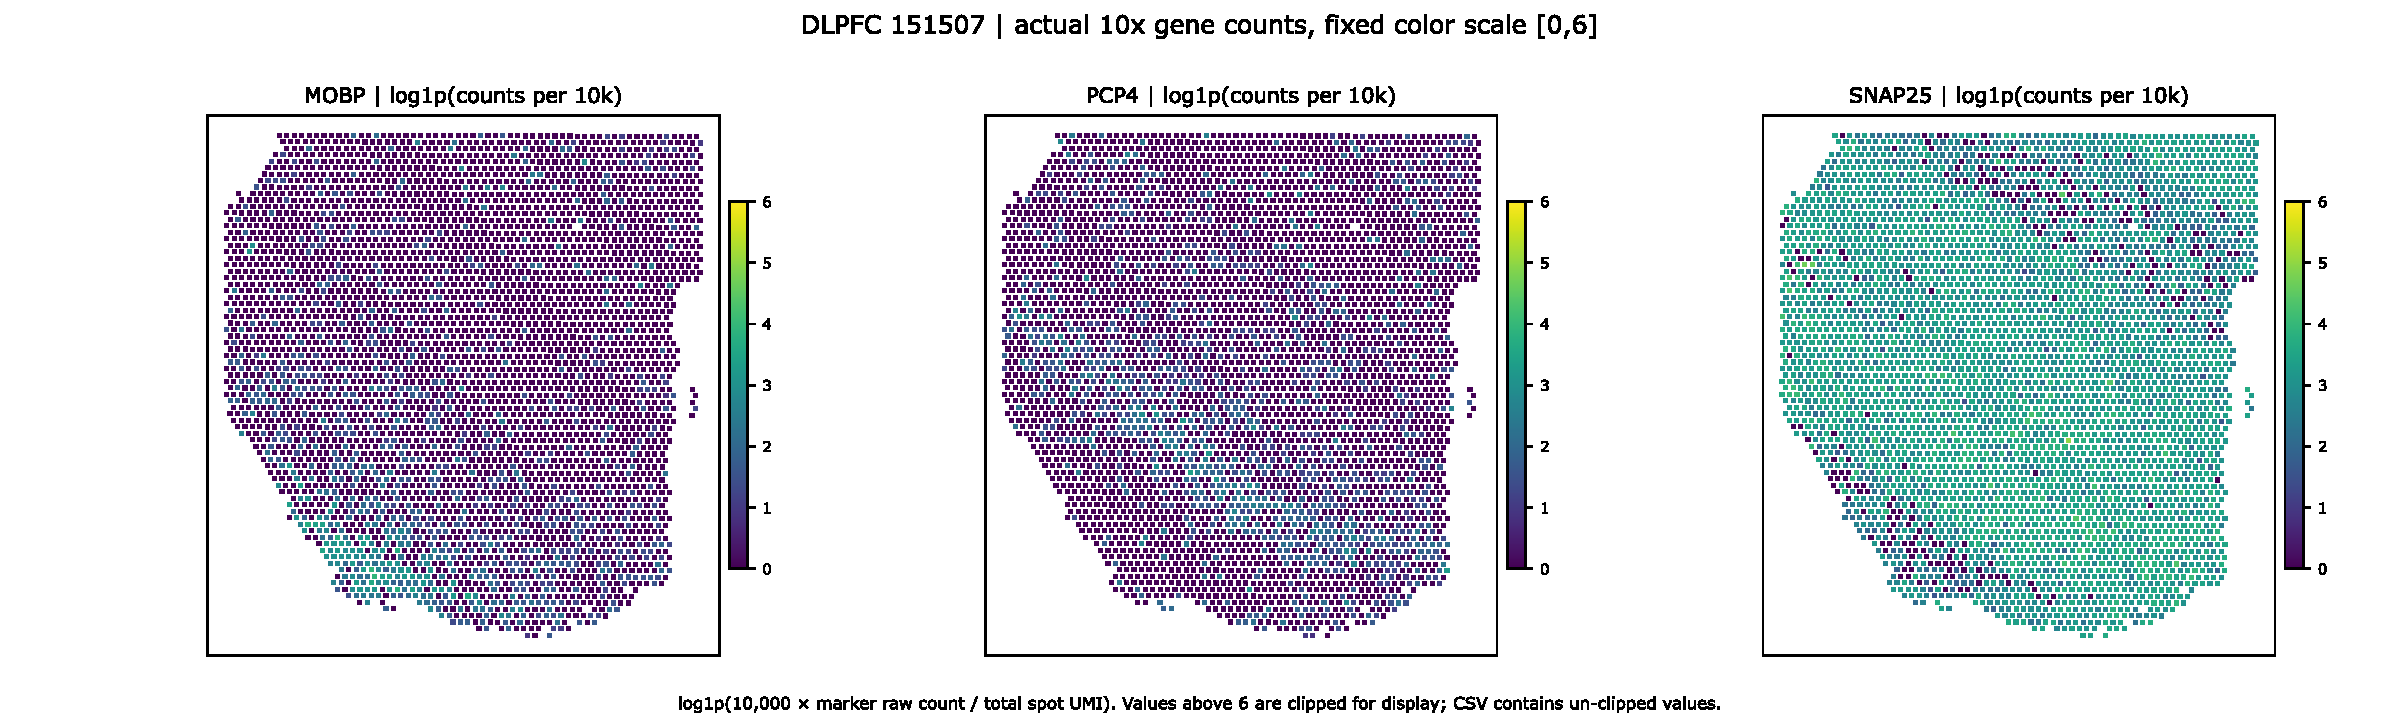
\includegraphics[width=0.97\linewidth,height=0.72\textheight,keepaspectratio]{E4_SOURCE_FIGURES_20261122_RELEASE/figures_pdf/151507/151507_MOBP_PCP4_SNAP25_expression.pdf}
\captionof{figure}{DLPFC切片151507：MOBP/PCP4/SNAP25表达三联图（原始E4图件转换的矢量PDF；聚类编号未根据参考标签重排）。}
\label{fig:cc-e4-app-151507-markers}
\end{minipage}\par\medskip
}{%
\par\noindent\emph{[编译提示：未找到该图件的PDF，请检查相对路径。]}\par
}
\IfFileExists{E4_SOURCE_FIGURES_20261122_RELEASE/figures_pdf/151507/151507_reference_A_B_confusion.pdf}{%
\par\noindent\begin{minipage}{\linewidth}
\centering
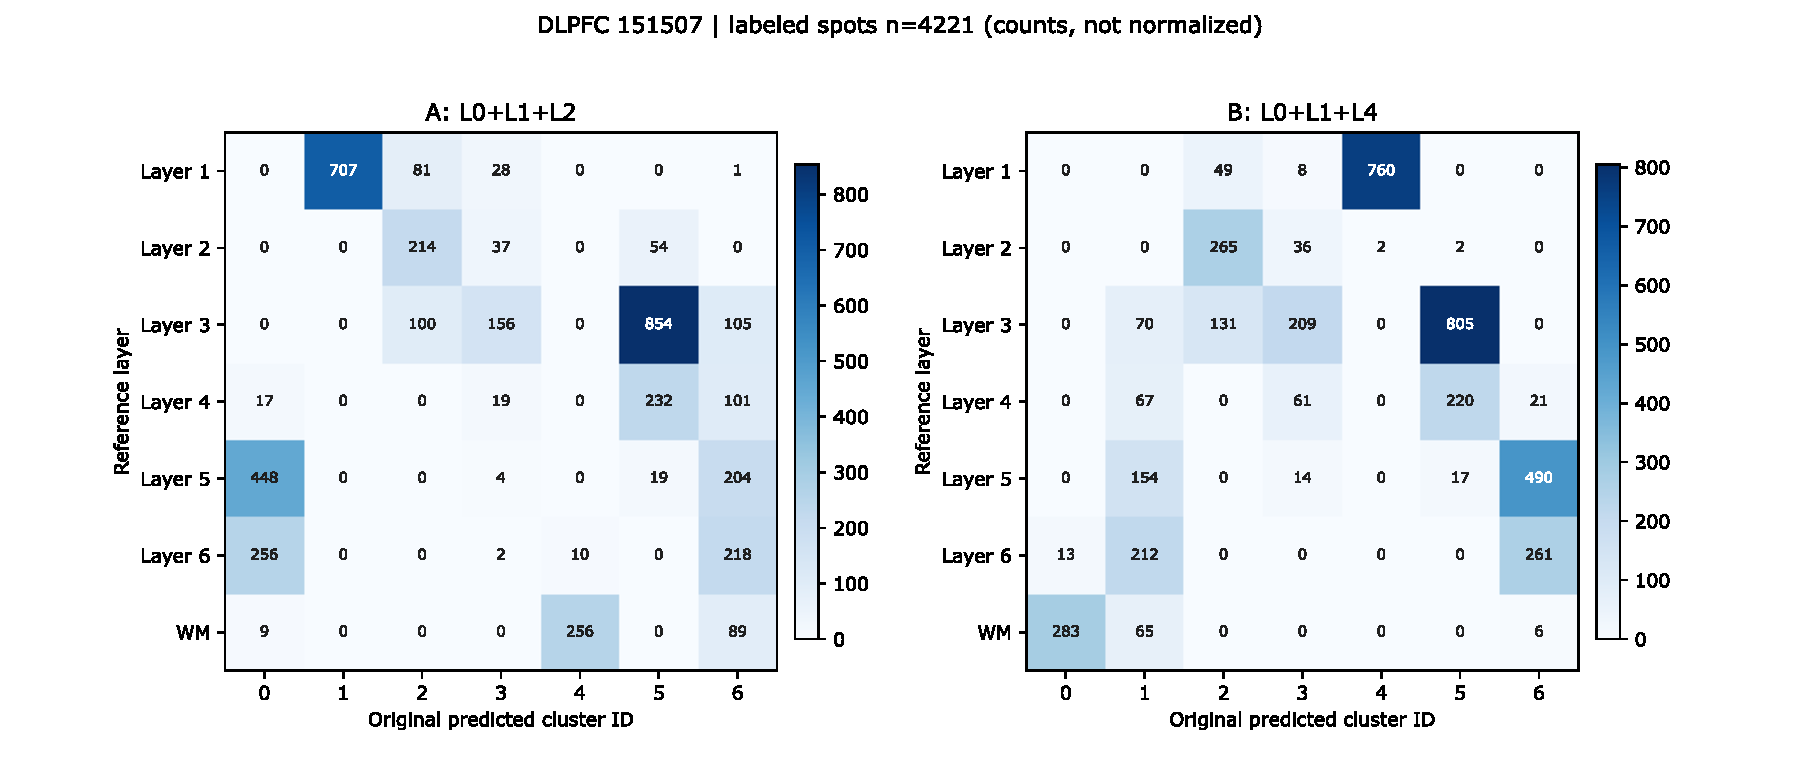
\includegraphics[width=0.97\linewidth,height=0.72\textheight,keepaspectratio]{E4_SOURCE_FIGURES_20261122_RELEASE/figures_pdf/151507/151507_reference_A_B_confusion.pdf}
\captionof{figure}{DLPFC切片151507：参考层与A/B簇交叉计数图（原始E4图件转换的矢量PDF；聚类编号未根据参考标签重排）。}
\label{fig:cc-e4-app-151507-confusion}
\end{minipage}\par\medskip
}{%
\par\noindent\emph{[编译提示：未找到该图件的PDF，请检查相对路径。]}\par
}
\subsection{DLPFC切片151508}
\IfFileExists{E4_SOURCE_FIGURES_20261122_RELEASE/figures_pdf/151508/151508_reference_A_B_spatial.pdf}{%
\par\noindent\begin{minipage}{\linewidth}
\centering
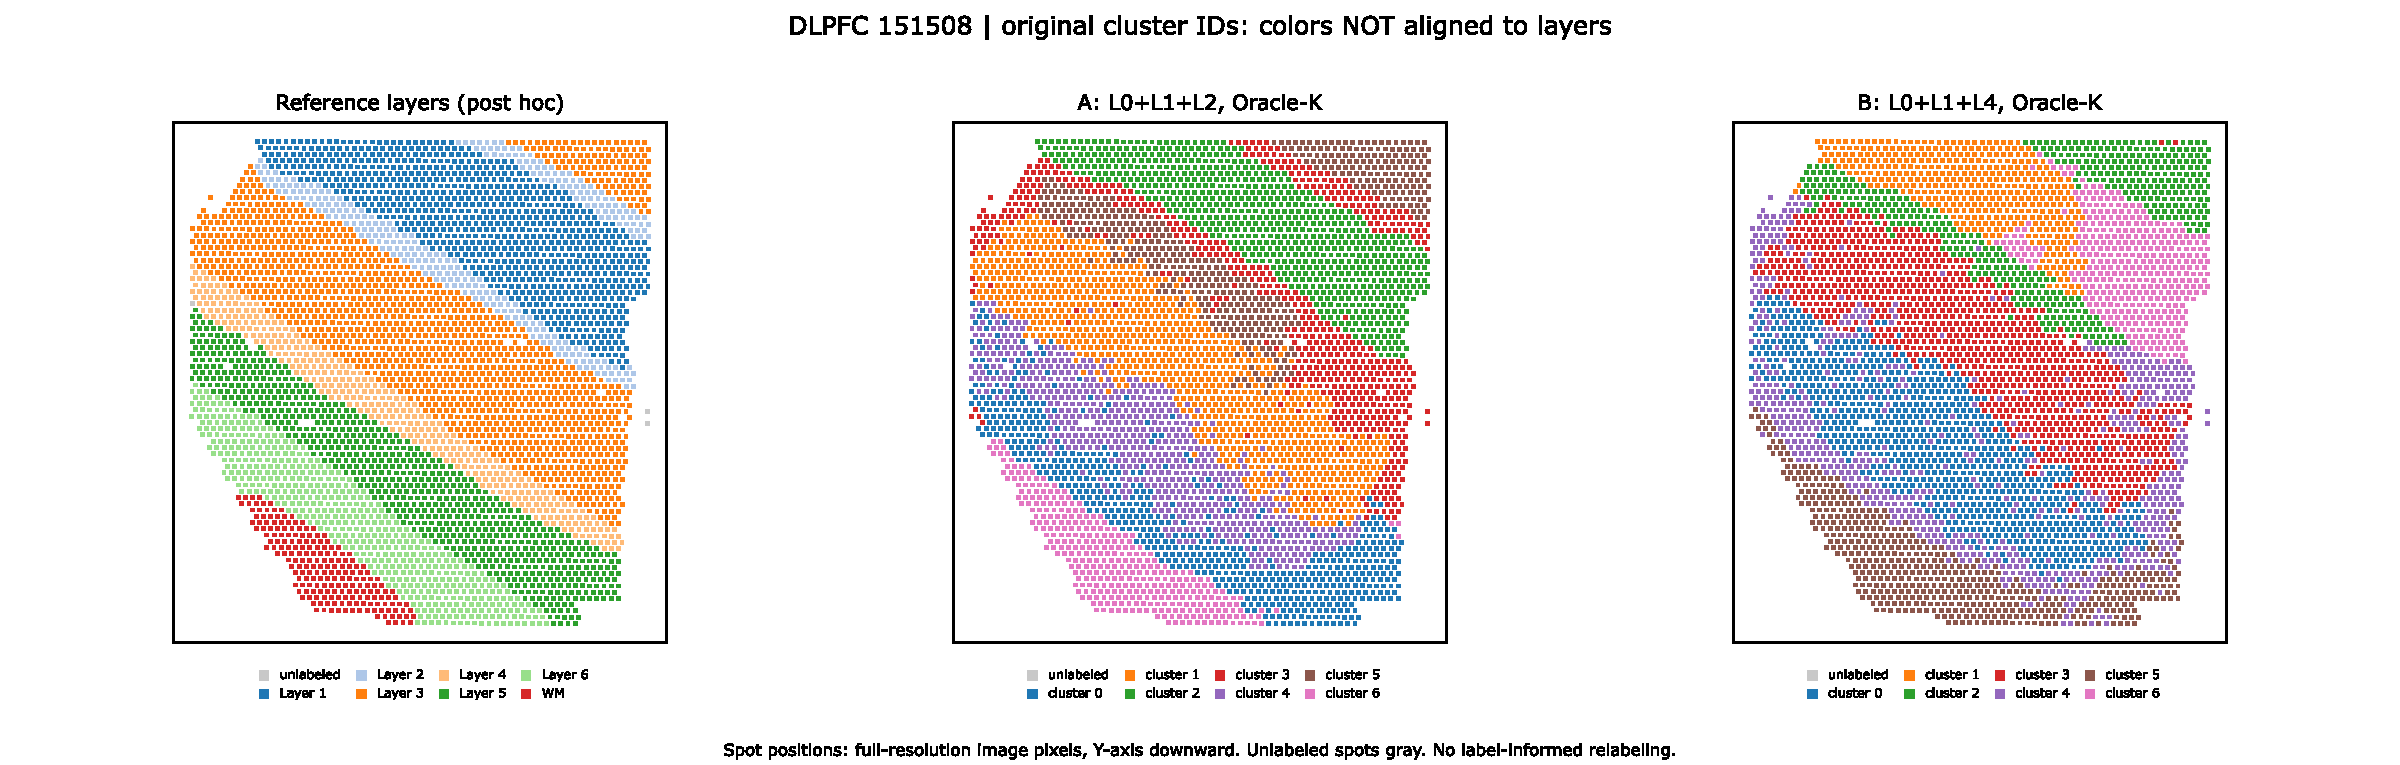
\includegraphics[width=0.97\linewidth,height=0.72\textheight,keepaspectratio]{E4_SOURCE_FIGURES_20261122_RELEASE/figures_pdf/151508/151508_reference_A_B_spatial.pdf}
\captionof{figure}{DLPFC切片151508：参考层与A/B原始聚类三联图（原始E4图件转换的矢量PDF；聚类编号未根据参考标签重排）。}
\label{fig:cc-e4-app-151508-map}
\end{minipage}\par\medskip
}{%
\par\noindent\emph{[编译提示：未找到该图件的PDF，请检查相对路径。]}\par
}
\IfFileExists{E4_SOURCE_FIGURES_20261122_RELEASE/figures_pdf/151508/151508_MOBP_PCP4_SNAP25_expression.pdf}{%
\par\noindent\begin{minipage}{\linewidth}
\centering
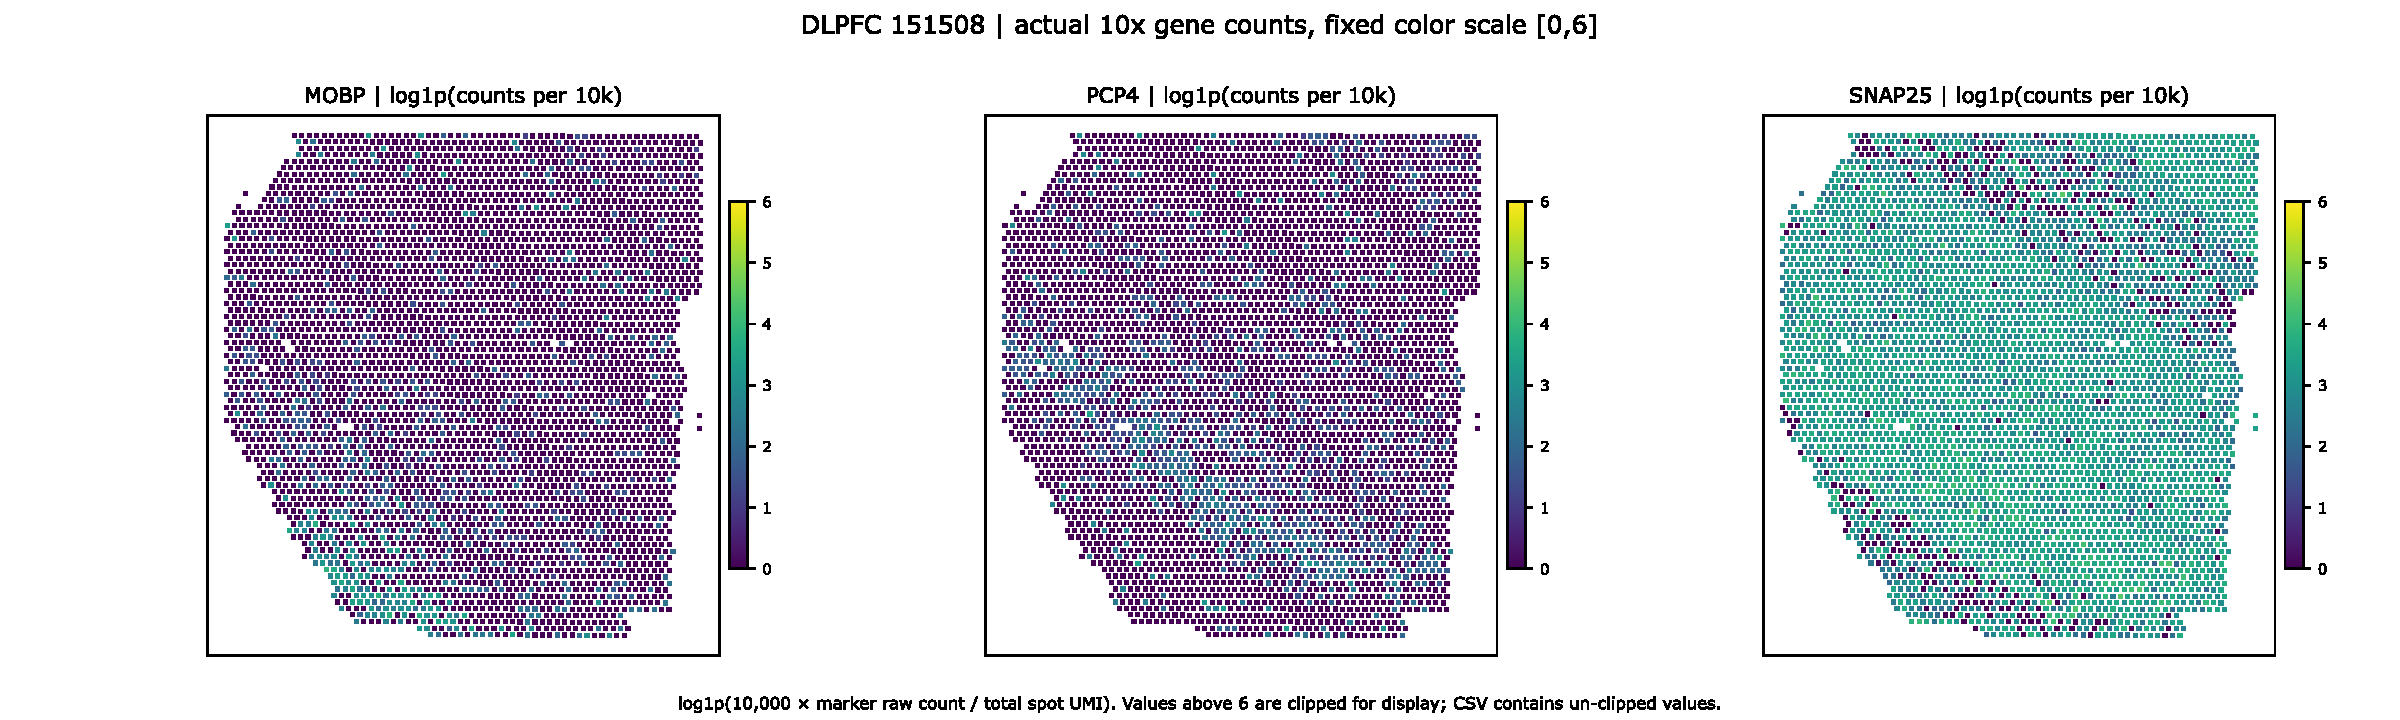
\includegraphics[width=0.97\linewidth,height=0.72\textheight,keepaspectratio]{E4_SOURCE_FIGURES_20261122_RELEASE/figures_pdf/151508/151508_MOBP_PCP4_SNAP25_expression.pdf}
\captionof{figure}{DLPFC切片151508：MOBP/PCP4/SNAP25表达三联图（原始E4图件转换的矢量PDF；聚类编号未根据参考标签重排）。}
\label{fig:cc-e4-app-151508-markers}
\end{minipage}\par\medskip
}{%
\par\noindent\emph{[编译提示：未找到该图件的PDF，请检查相对路径。]}\par
}
\IfFileExists{E4_SOURCE_FIGURES_20261122_RELEASE/figures_pdf/151508/151508_reference_A_B_confusion.pdf}{%
\par\noindent\begin{minipage}{\linewidth}
\centering
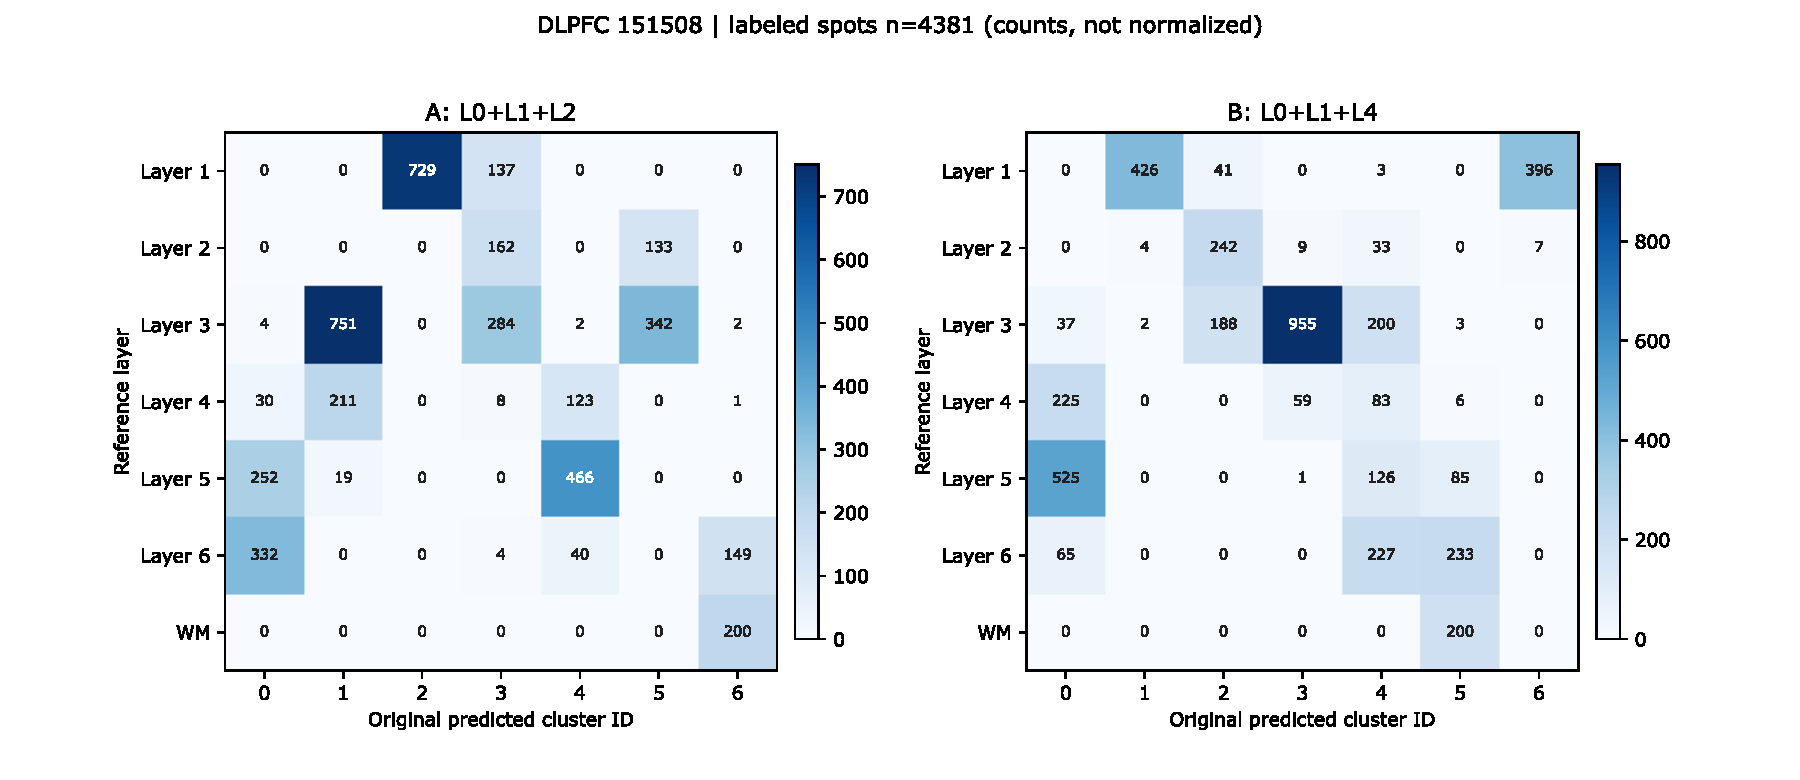
\includegraphics[width=0.97\linewidth,height=0.72\textheight,keepaspectratio]{E4_SOURCE_FIGURES_20261122_RELEASE/figures_pdf/151508/151508_reference_A_B_confusion.pdf}
\captionof{figure}{DLPFC切片151508：参考层与A/B簇交叉计数图（原始E4图件转换的矢量PDF；聚类编号未根据参考标签重排）。}
\label{fig:cc-e4-app-151508-confusion}
\end{minipage}\par\medskip
}{%
\par\noindent\emph{[编译提示：未找到该图件的PDF，请检查相对路径。]}\par
}
\subsection{DLPFC切片151509}
\IfFileExists{E4_SOURCE_FIGURES_20261122_RELEASE/figures_pdf/151509/151509_reference_A_B_spatial.pdf}{%
\par\noindent\begin{minipage}{\linewidth}
\centering
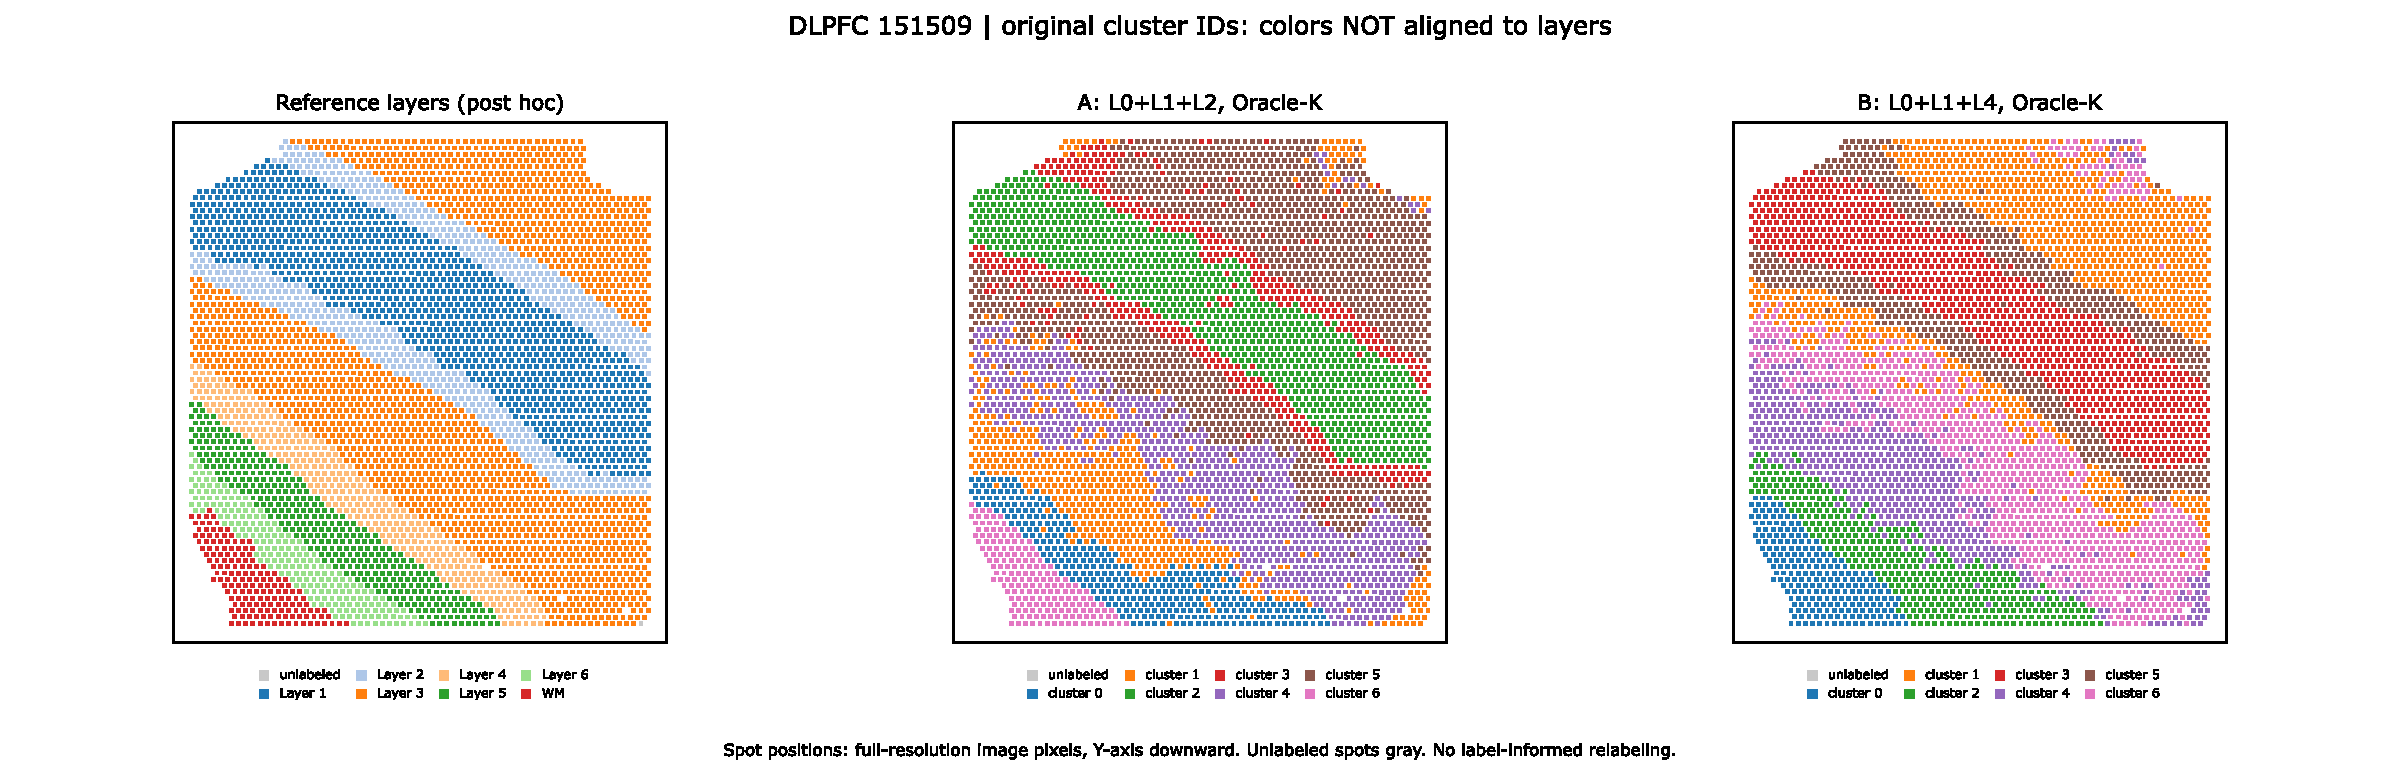
\includegraphics[width=0.97\linewidth,height=0.72\textheight,keepaspectratio]{E4_SOURCE_FIGURES_20261122_RELEASE/figures_pdf/151509/151509_reference_A_B_spatial.pdf}
\captionof{figure}{DLPFC切片151509：参考层与A/B原始聚类三联图（原始E4图件转换的矢量PDF；聚类编号未根据参考标签重排）。}
\label{fig:cc-e4-app-151509-map}
\end{minipage}\par\medskip
}{%
\par\noindent\emph{[编译提示：未找到该图件的PDF，请检查相对路径。]}\par
}
\IfFileExists{E4_SOURCE_FIGURES_20261122_RELEASE/figures_pdf/151509/151509_MOBP_PCP4_SNAP25_expression.pdf}{%
\par\noindent\begin{minipage}{\linewidth}
\centering
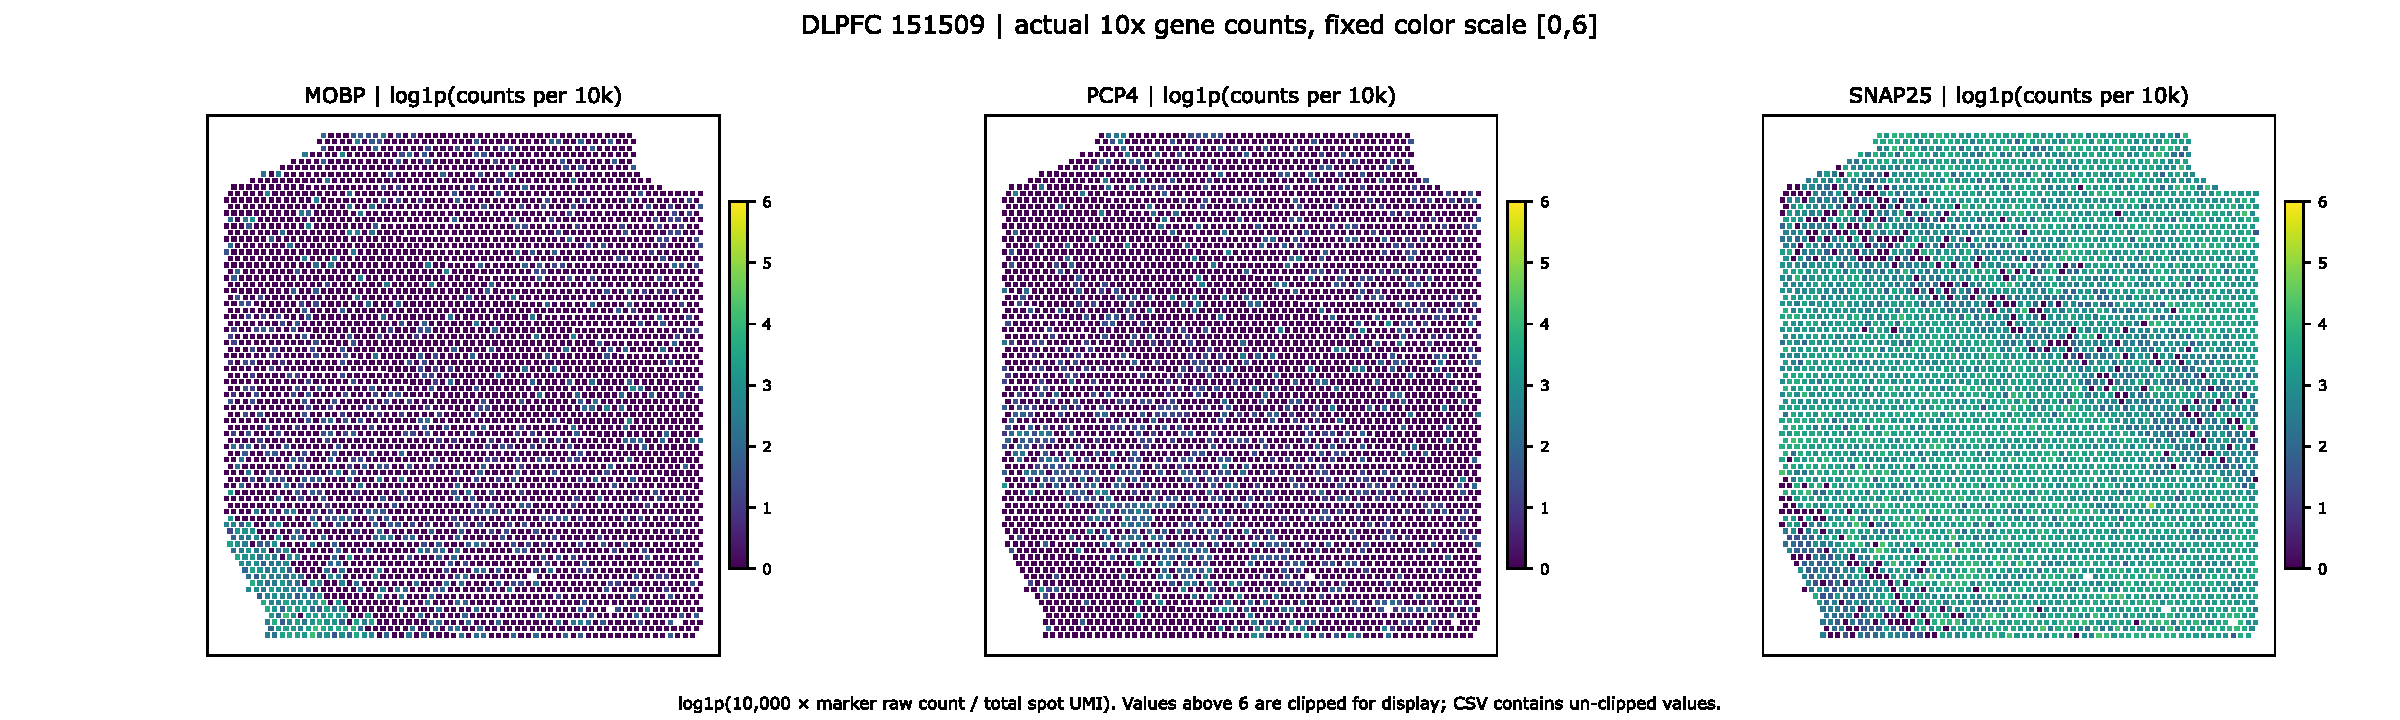
\includegraphics[width=0.97\linewidth,height=0.72\textheight,keepaspectratio]{E4_SOURCE_FIGURES_20261122_RELEASE/figures_pdf/151509/151509_MOBP_PCP4_SNAP25_expression.pdf}
\captionof{figure}{DLPFC切片151509：MOBP/PCP4/SNAP25表达三联图（原始E4图件转换的矢量PDF；聚类编号未根据参考标签重排）。}
\label{fig:cc-e4-app-151509-markers}
\end{minipage}\par\medskip
}{%
\par\noindent\emph{[编译提示：未找到该图件的PDF，请检查相对路径。]}\par
}
\IfFileExists{E4_SOURCE_FIGURES_20261122_RELEASE/figures_pdf/151509/151509_reference_A_B_confusion.pdf}{%
\par\noindent\begin{minipage}{\linewidth}
\centering
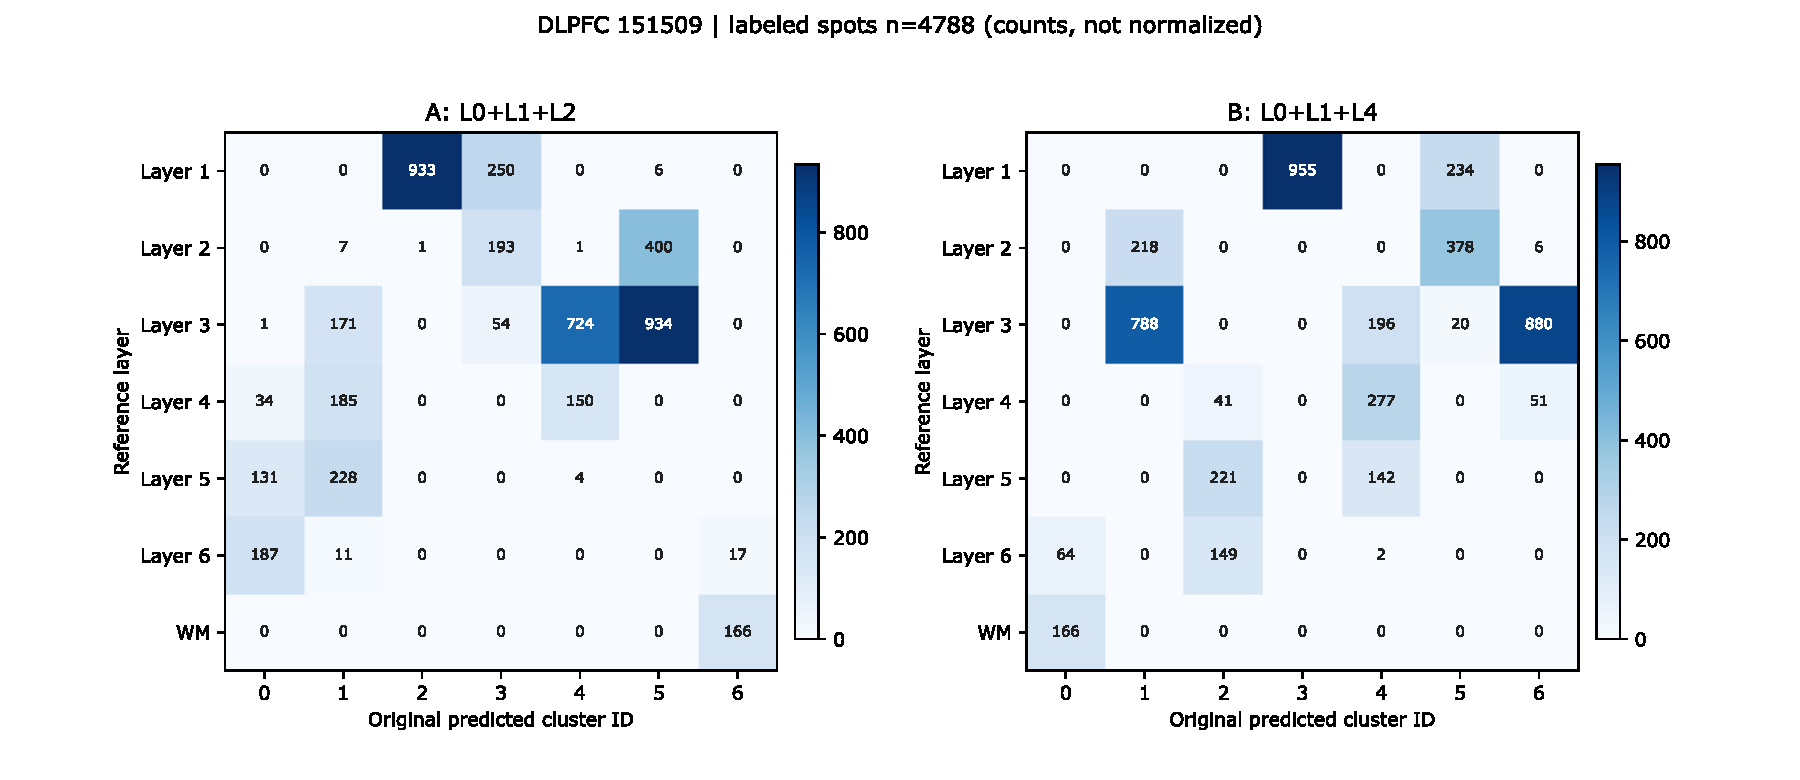
\includegraphics[width=0.97\linewidth,height=0.72\textheight,keepaspectratio]{E4_SOURCE_FIGURES_20261122_RELEASE/figures_pdf/151509/151509_reference_A_B_confusion.pdf}
\captionof{figure}{DLPFC切片151509：参考层与A/B簇交叉计数图（原始E4图件转换的矢量PDF；聚类编号未根据参考标签重排）。}
\label{fig:cc-e4-app-151509-confusion}
\end{minipage}\par\medskip
}{%
\par\noindent\emph{[编译提示：未找到该图件的PDF，请检查相对路径。]}\par
}
\subsection{DLPFC切片151510}
\IfFileExists{E4_SOURCE_FIGURES_20261122_RELEASE/figures_pdf/151510/151510_reference_A_B_spatial.pdf}{%
\par\noindent\begin{minipage}{\linewidth}
\centering
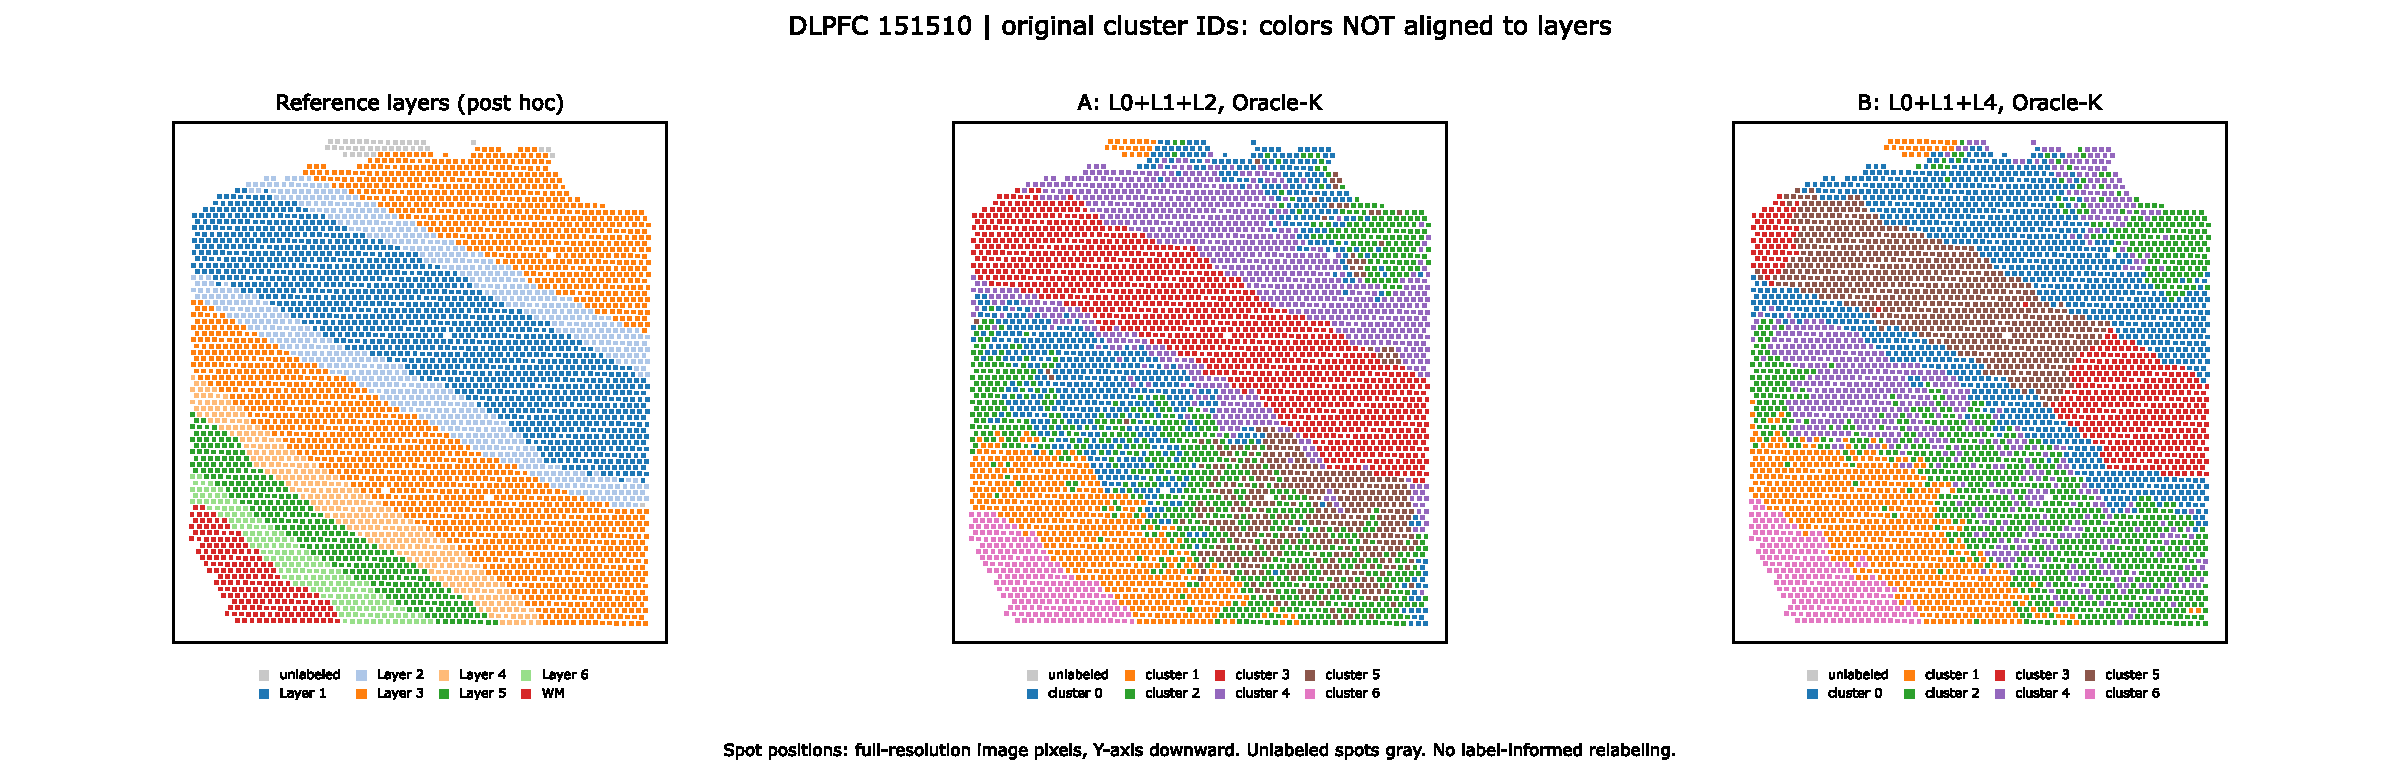
\includegraphics[width=0.97\linewidth,height=0.72\textheight,keepaspectratio]{E4_SOURCE_FIGURES_20261122_RELEASE/figures_pdf/151510/151510_reference_A_B_spatial.pdf}
\captionof{figure}{DLPFC切片151510：参考层与A/B原始聚类三联图（原始E4图件转换的矢量PDF；聚类编号未根据参考标签重排）。}
\label{fig:cc-e4-app-151510-map}
\end{minipage}\par\medskip
}{%
\par\noindent\emph{[编译提示：未找到该图件的PDF，请检查相对路径。]}\par
}
\IfFileExists{E4_SOURCE_FIGURES_20261122_RELEASE/figures_pdf/151510/151510_MOBP_PCP4_SNAP25_expression.pdf}{%
\par\noindent\begin{minipage}{\linewidth}
\centering
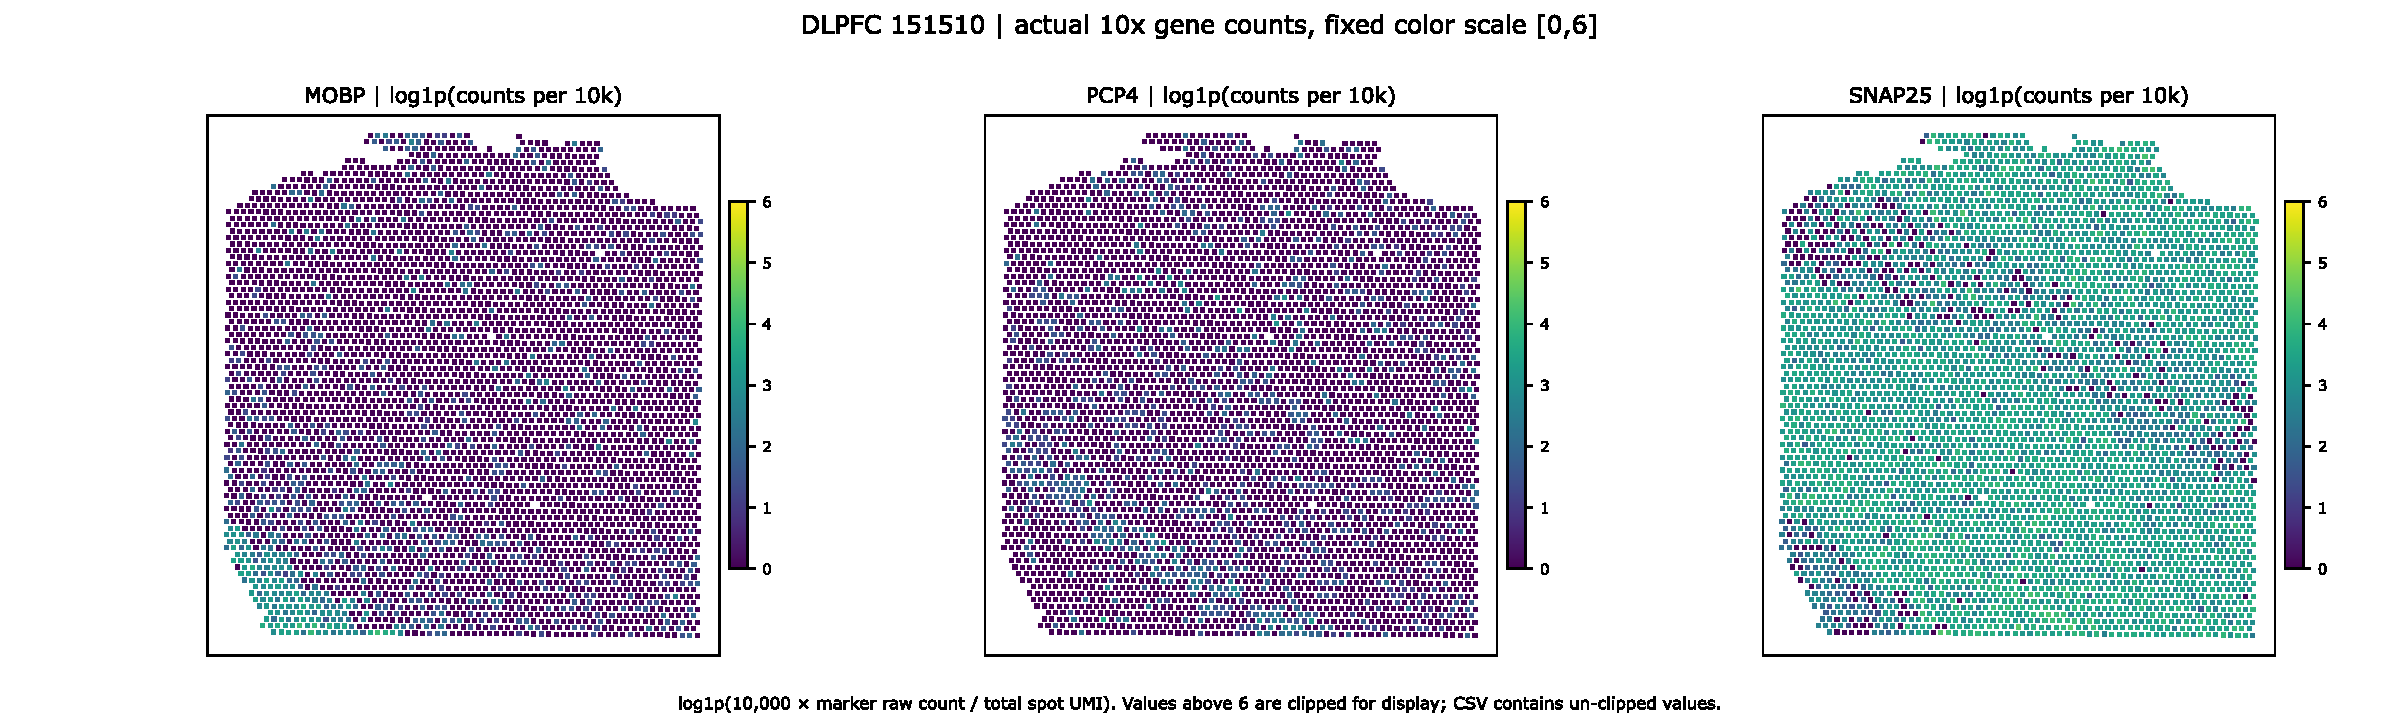
\includegraphics[width=0.97\linewidth,height=0.72\textheight,keepaspectratio]{E4_SOURCE_FIGURES_20261122_RELEASE/figures_pdf/151510/151510_MOBP_PCP4_SNAP25_expression.pdf}
\captionof{figure}{DLPFC切片151510：MOBP/PCP4/SNAP25表达三联图（原始E4图件转换的矢量PDF；聚类编号未根据参考标签重排）。}
\label{fig:cc-e4-app-151510-markers}
\end{minipage}\par\medskip
}{%
\par\noindent\emph{[编译提示：未找到该图件的PDF，请检查相对路径。]}\par
}
\IfFileExists{E4_SOURCE_FIGURES_20261122_RELEASE/figures_pdf/151510/151510_reference_A_B_confusion.pdf}{%
\par\noindent\begin{minipage}{\linewidth}
\centering
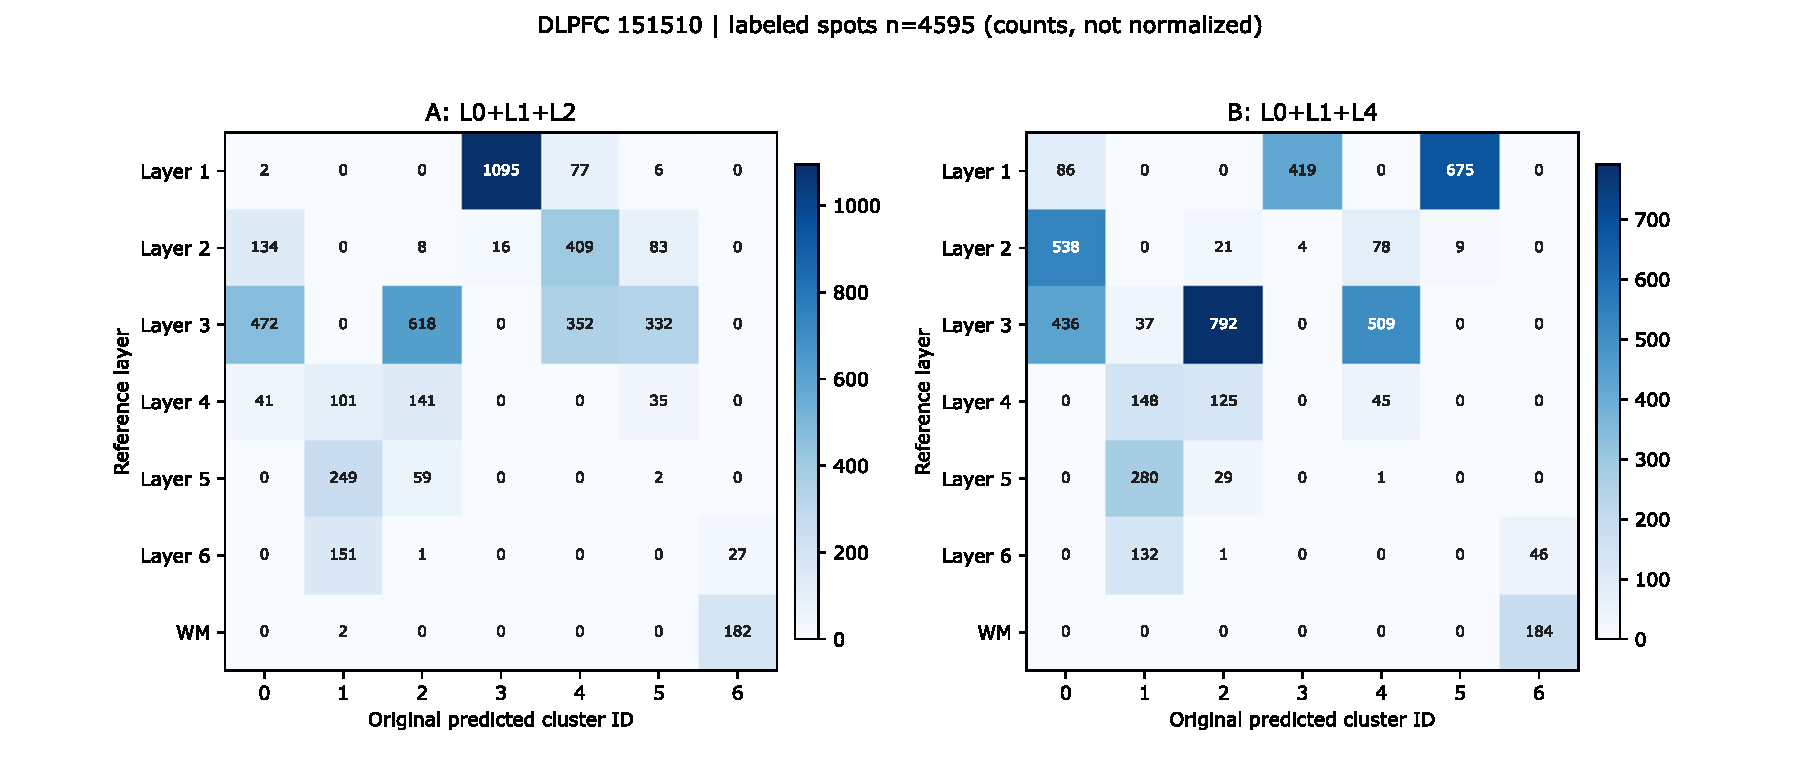
\includegraphics[width=0.97\linewidth,height=0.72\textheight,keepaspectratio]{E4_SOURCE_FIGURES_20261122_RELEASE/figures_pdf/151510/151510_reference_A_B_confusion.pdf}
\captionof{figure}{DLPFC切片151510：参考层与A/B簇交叉计数图（原始E4图件转换的矢量PDF；聚类编号未根据参考标签重排）。}
\label{fig:cc-e4-app-151510-confusion}
\end{minipage}\par\medskip
}{%
\par\noindent\emph{[编译提示：未找到该图件的PDF，请检查相对路径。]}\par
}
\subsection{DLPFC切片151669}
\IfFileExists{E4_SOURCE_FIGURES_20261122_RELEASE/figures_pdf/151669/151669_reference_A_B_spatial.pdf}{%
\par\noindent\begin{minipage}{\linewidth}
\centering
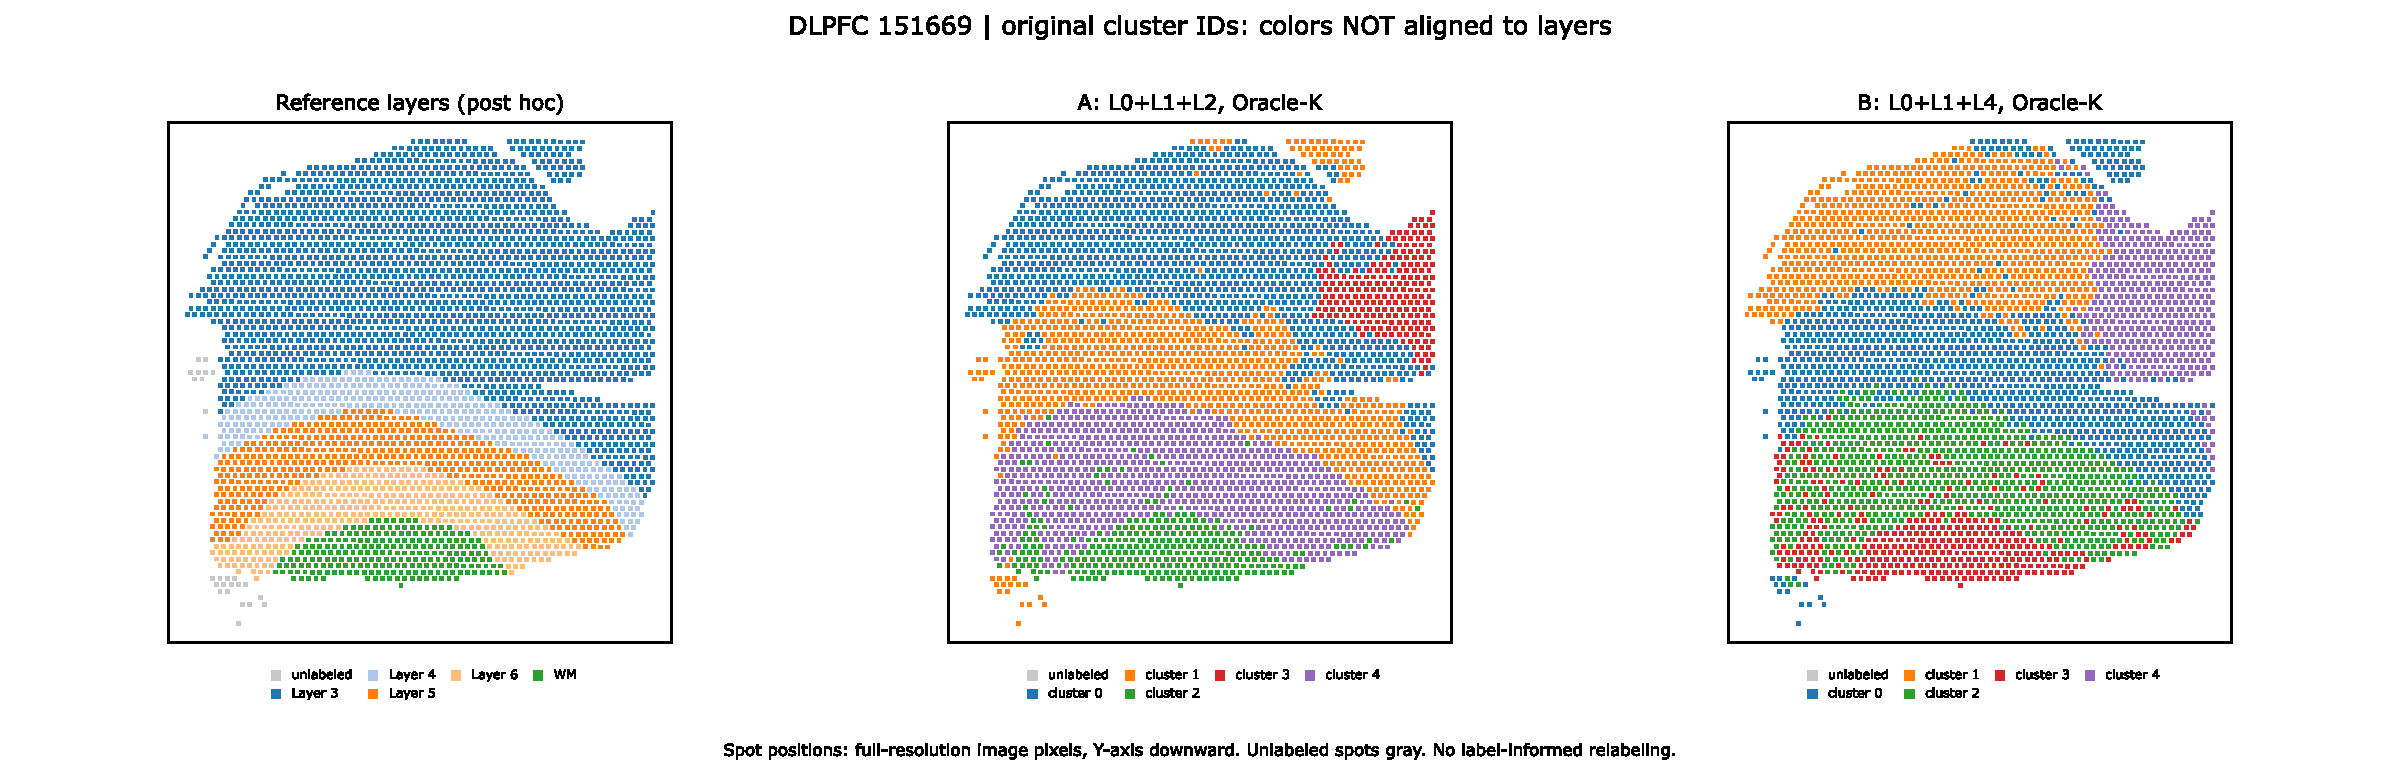
\includegraphics[width=0.97\linewidth,height=0.72\textheight,keepaspectratio]{E4_SOURCE_FIGURES_20261122_RELEASE/figures_pdf/151669/151669_reference_A_B_spatial.pdf}
\captionof{figure}{DLPFC切片151669：参考层与A/B原始聚类三联图（原始E4图件转换的矢量PDF；聚类编号未根据参考标签重排）。}
\label{fig:cc-e4-app-151669-map}
\end{minipage}\par\medskip
}{%
\par\noindent\emph{[编译提示：未找到该图件的PDF，请检查相对路径。]}\par
}
\IfFileExists{E4_SOURCE_FIGURES_20261122_RELEASE/figures_pdf/151669/151669_MOBP_PCP4_SNAP25_expression.pdf}{%
\par\noindent\begin{minipage}{\linewidth}
\centering
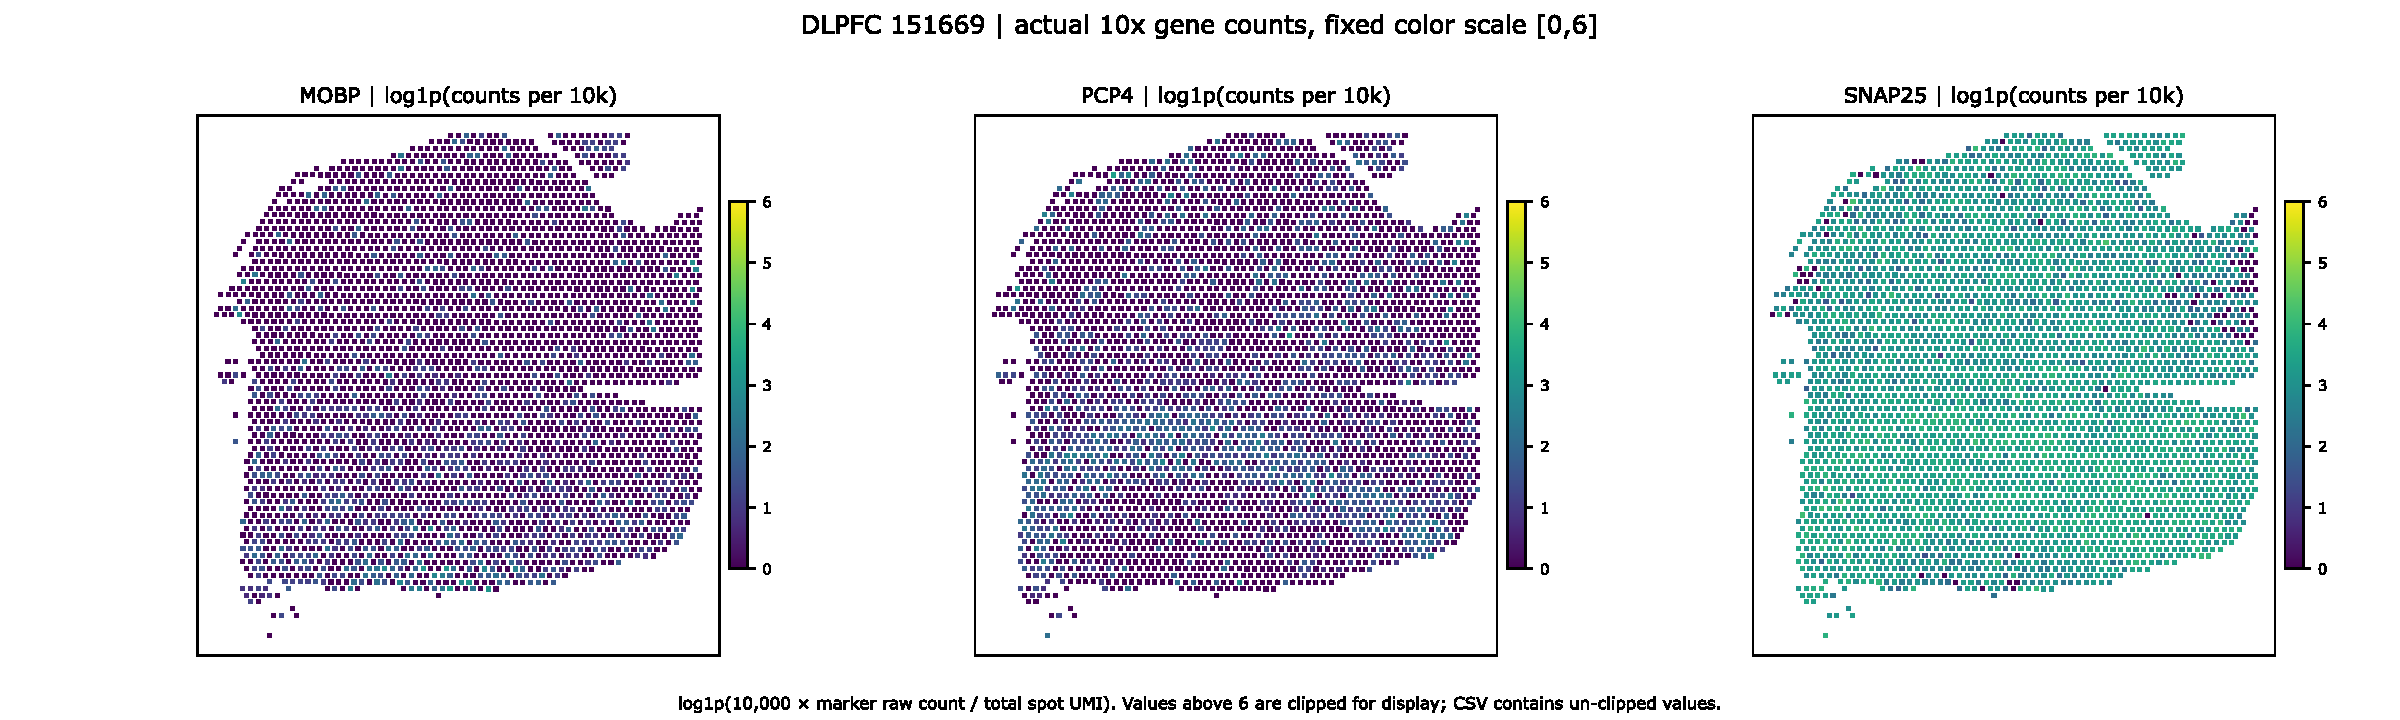
\includegraphics[width=0.97\linewidth,height=0.72\textheight,keepaspectratio]{E4_SOURCE_FIGURES_20261122_RELEASE/figures_pdf/151669/151669_MOBP_PCP4_SNAP25_expression.pdf}
\captionof{figure}{DLPFC切片151669：MOBP/PCP4/SNAP25表达三联图（原始E4图件转换的矢量PDF；聚类编号未根据参考标签重排）。}
\label{fig:cc-e4-app-151669-markers}
\end{minipage}\par\medskip
}{%
\par\noindent\emph{[编译提示：未找到该图件的PDF，请检查相对路径。]}\par
}
\IfFileExists{E4_SOURCE_FIGURES_20261122_RELEASE/figures_pdf/151669/151669_reference_A_B_confusion.pdf}{%
\par\noindent\begin{minipage}{\linewidth}
\centering
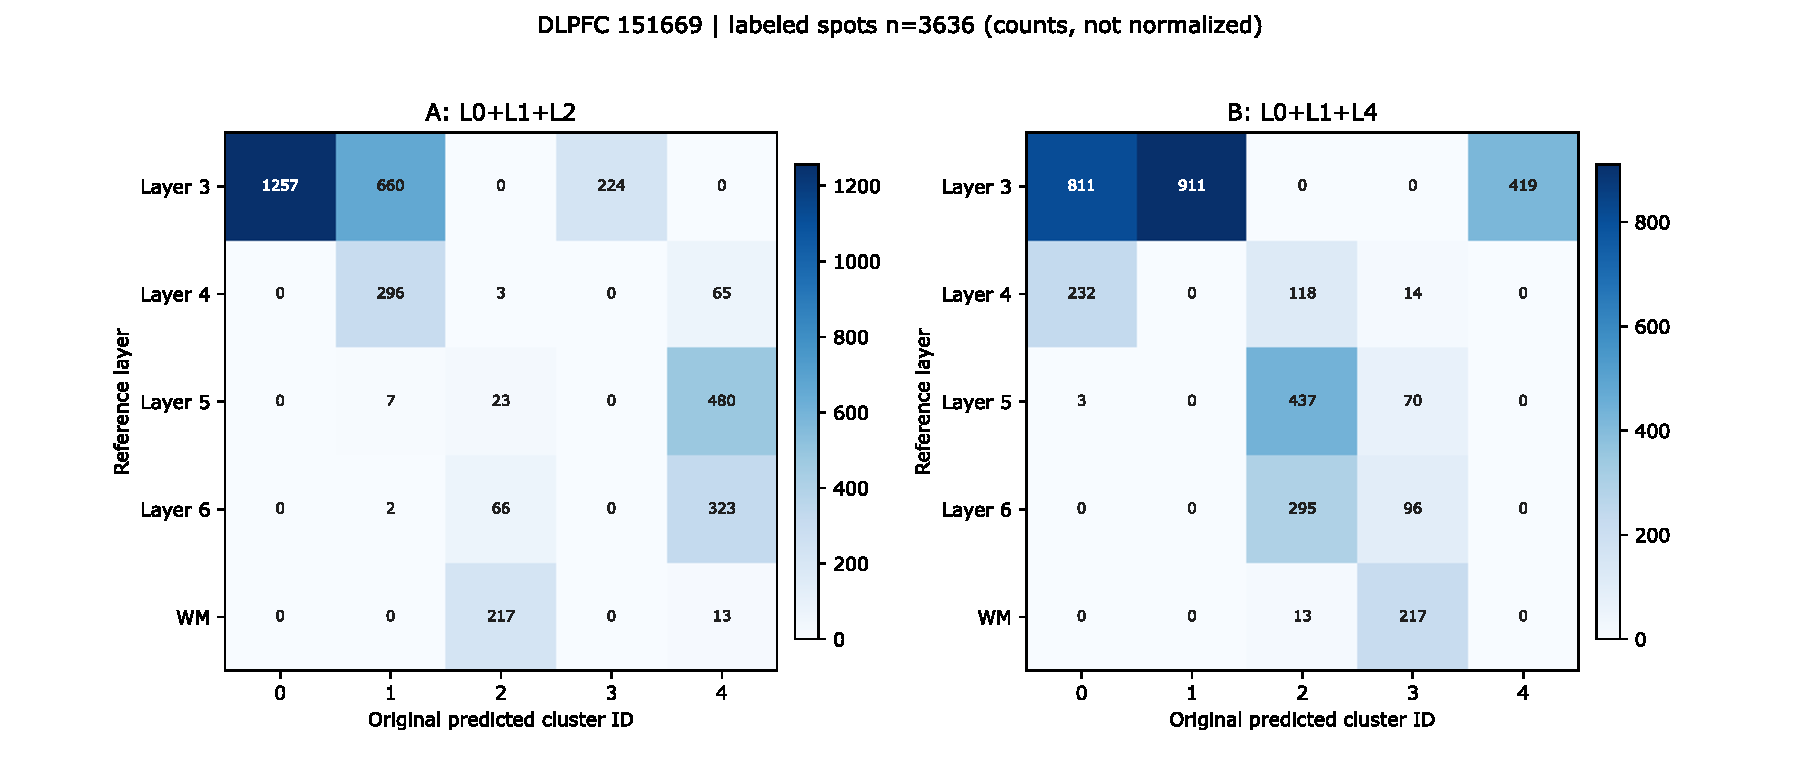
\includegraphics[width=0.97\linewidth,height=0.72\textheight,keepaspectratio]{E4_SOURCE_FIGURES_20261122_RELEASE/figures_pdf/151669/151669_reference_A_B_confusion.pdf}
\captionof{figure}{DLPFC切片151669：参考层与A/B簇交叉计数图（原始E4图件转换的矢量PDF；聚类编号未根据参考标签重排）。}
\label{fig:cc-e4-app-151669-confusion}
\end{minipage}\par\medskip
}{%
\par\noindent\emph{[编译提示：未找到该图件的PDF，请检查相对路径。]}\par
}
\subsection{DLPFC切片151670}
\IfFileExists{E4_SOURCE_FIGURES_20261122_RELEASE/figures_pdf/151670/151670_reference_A_B_spatial.pdf}{%
\par\noindent\begin{minipage}{\linewidth}
\centering
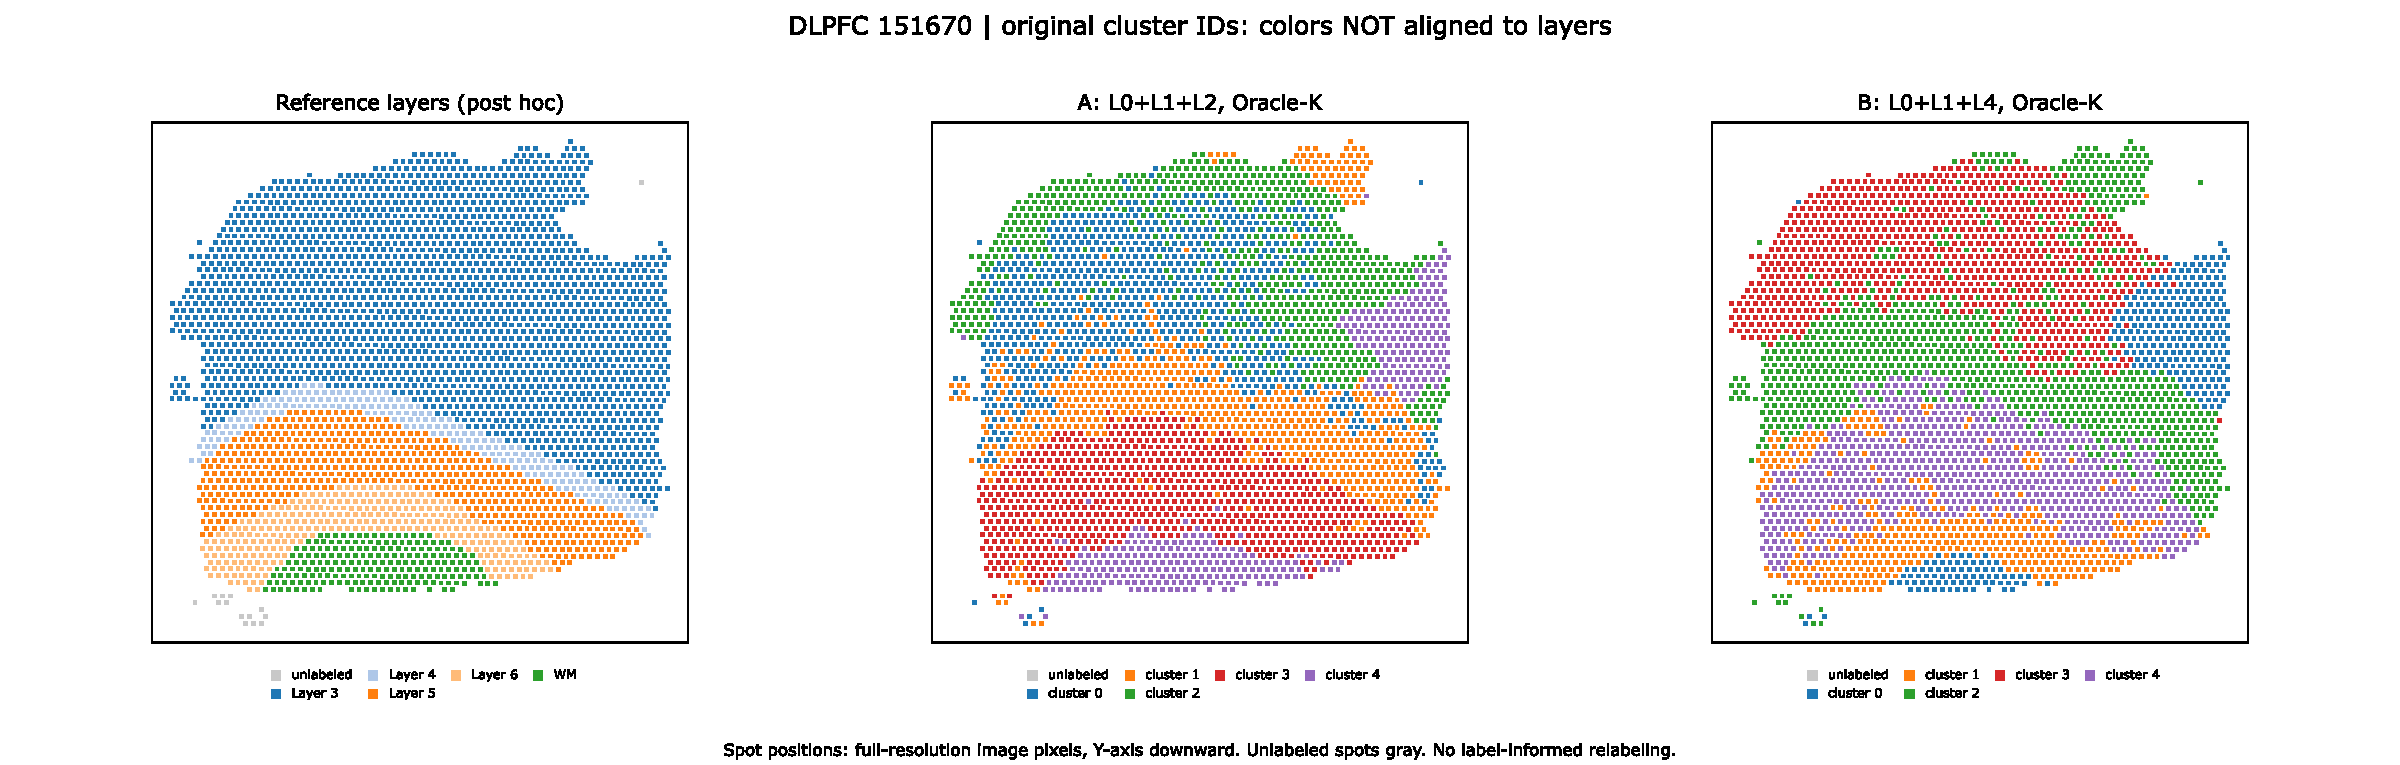
\includegraphics[width=0.97\linewidth,height=0.72\textheight,keepaspectratio]{E4_SOURCE_FIGURES_20261122_RELEASE/figures_pdf/151670/151670_reference_A_B_spatial.pdf}
\captionof{figure}{DLPFC切片151670：参考层与A/B原始聚类三联图（原始E4图件转换的矢量PDF；聚类编号未根据参考标签重排）。}
\label{fig:cc-e4-app-151670-map}
\end{minipage}\par\medskip
}{%
\par\noindent\emph{[编译提示：未找到该图件的PDF，请检查相对路径。]}\par
}
\IfFileExists{E4_SOURCE_FIGURES_20261122_RELEASE/figures_pdf/151670/151670_MOBP_PCP4_SNAP25_expression.pdf}{%
\par\noindent\begin{minipage}{\linewidth}
\centering
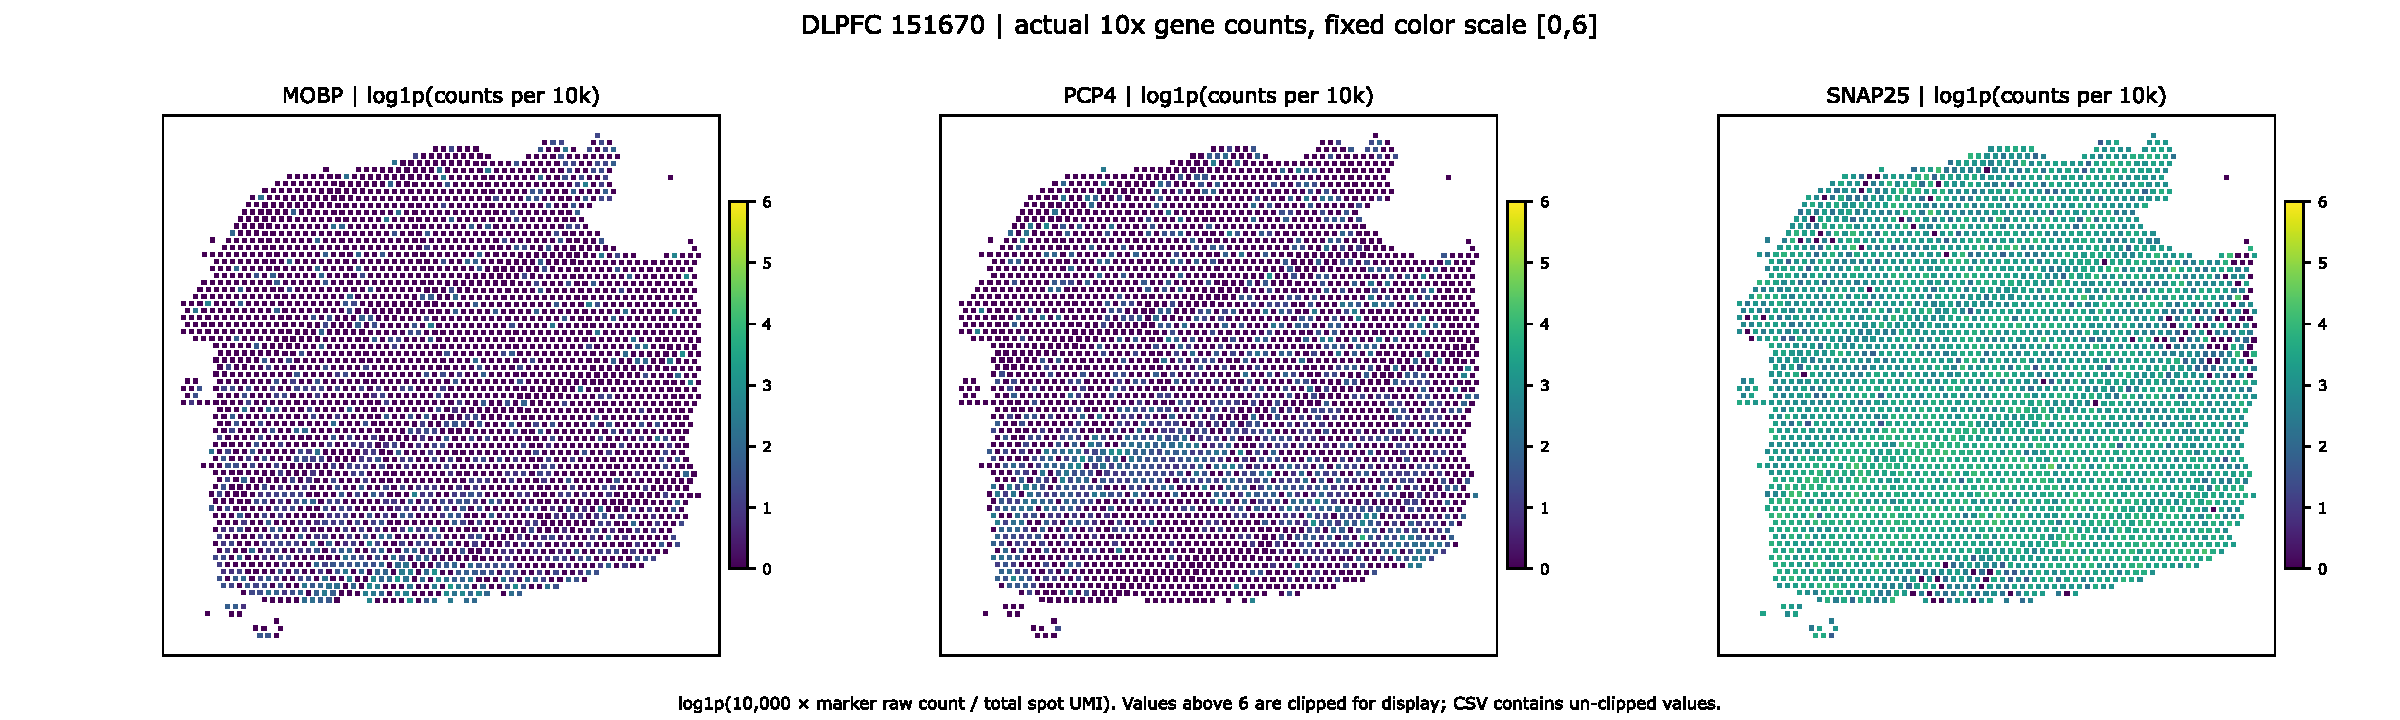
\includegraphics[width=0.97\linewidth,height=0.72\textheight,keepaspectratio]{E4_SOURCE_FIGURES_20261122_RELEASE/figures_pdf/151670/151670_MOBP_PCP4_SNAP25_expression.pdf}
\captionof{figure}{DLPFC切片151670：MOBP/PCP4/SNAP25表达三联图（原始E4图件转换的矢量PDF；聚类编号未根据参考标签重排）。}
\label{fig:cc-e4-app-151670-markers}
\end{minipage}\par\medskip
}{%
\par\noindent\emph{[编译提示：未找到该图件的PDF，请检查相对路径。]}\par
}
\IfFileExists{E4_SOURCE_FIGURES_20261122_RELEASE/figures_pdf/151670/151670_reference_A_B_confusion.pdf}{%
\par\noindent\begin{minipage}{\linewidth}
\centering
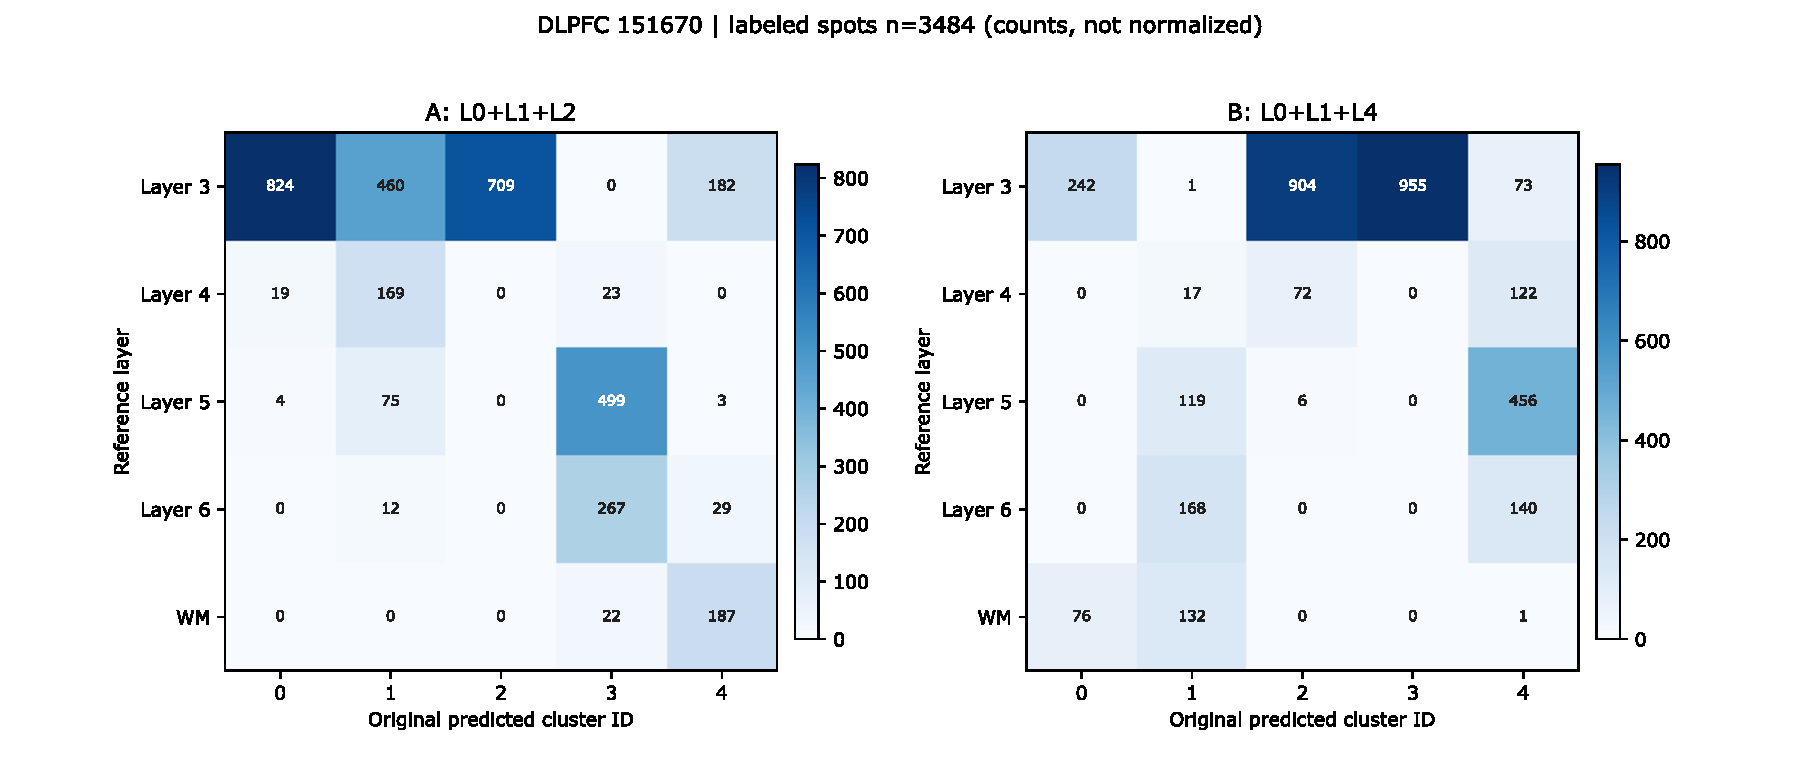
\includegraphics[width=0.97\linewidth,height=0.72\textheight,keepaspectratio]{E4_SOURCE_FIGURES_20261122_RELEASE/figures_pdf/151670/151670_reference_A_B_confusion.pdf}
\captionof{figure}{DLPFC切片151670：参考层与A/B簇交叉计数图（原始E4图件转换的矢量PDF；聚类编号未根据参考标签重排）。}
\label{fig:cc-e4-app-151670-confusion}
\end{minipage}\par\medskip
}{%
\par\noindent\emph{[编译提示：未找到该图件的PDF，请检查相对路径。]}\par
}
\subsection{DLPFC切片151671}
\IfFileExists{E4_SOURCE_FIGURES_20261122_RELEASE/figures_pdf/151671/151671_reference_A_B_spatial.pdf}{%
\par\noindent\begin{minipage}{\linewidth}
\centering
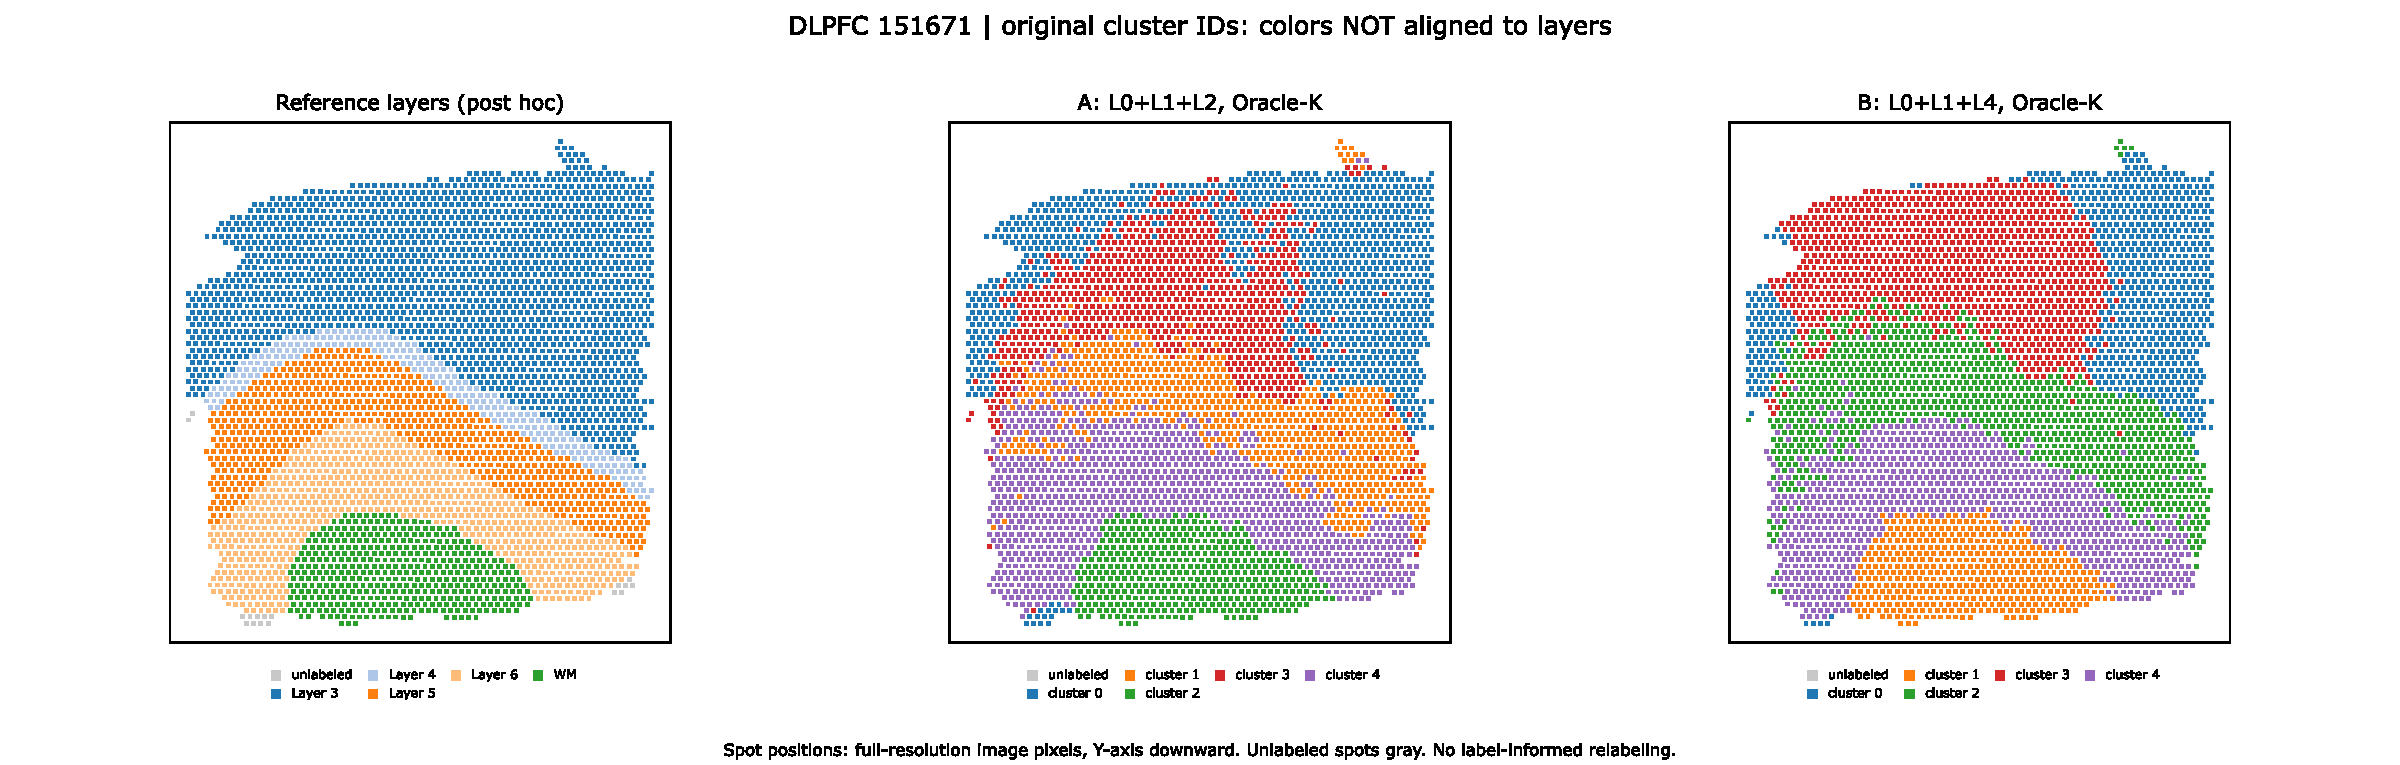
\includegraphics[width=0.97\linewidth,height=0.72\textheight,keepaspectratio]{E4_SOURCE_FIGURES_20261122_RELEASE/figures_pdf/151671/151671_reference_A_B_spatial.pdf}
\captionof{figure}{DLPFC切片151671：参考层与A/B原始聚类三联图（原始E4图件转换的矢量PDF；聚类编号未根据参考标签重排）。}
\label{fig:cc-e4-app-151671-map}
\end{minipage}\par\medskip
}{%
\par\noindent\emph{[编译提示：未找到该图件的PDF，请检查相对路径。]}\par
}
\IfFileExists{E4_SOURCE_FIGURES_20261122_RELEASE/figures_pdf/151671/151671_MOBP_PCP4_SNAP25_expression.pdf}{%
\par\noindent\begin{minipage}{\linewidth}
\centering
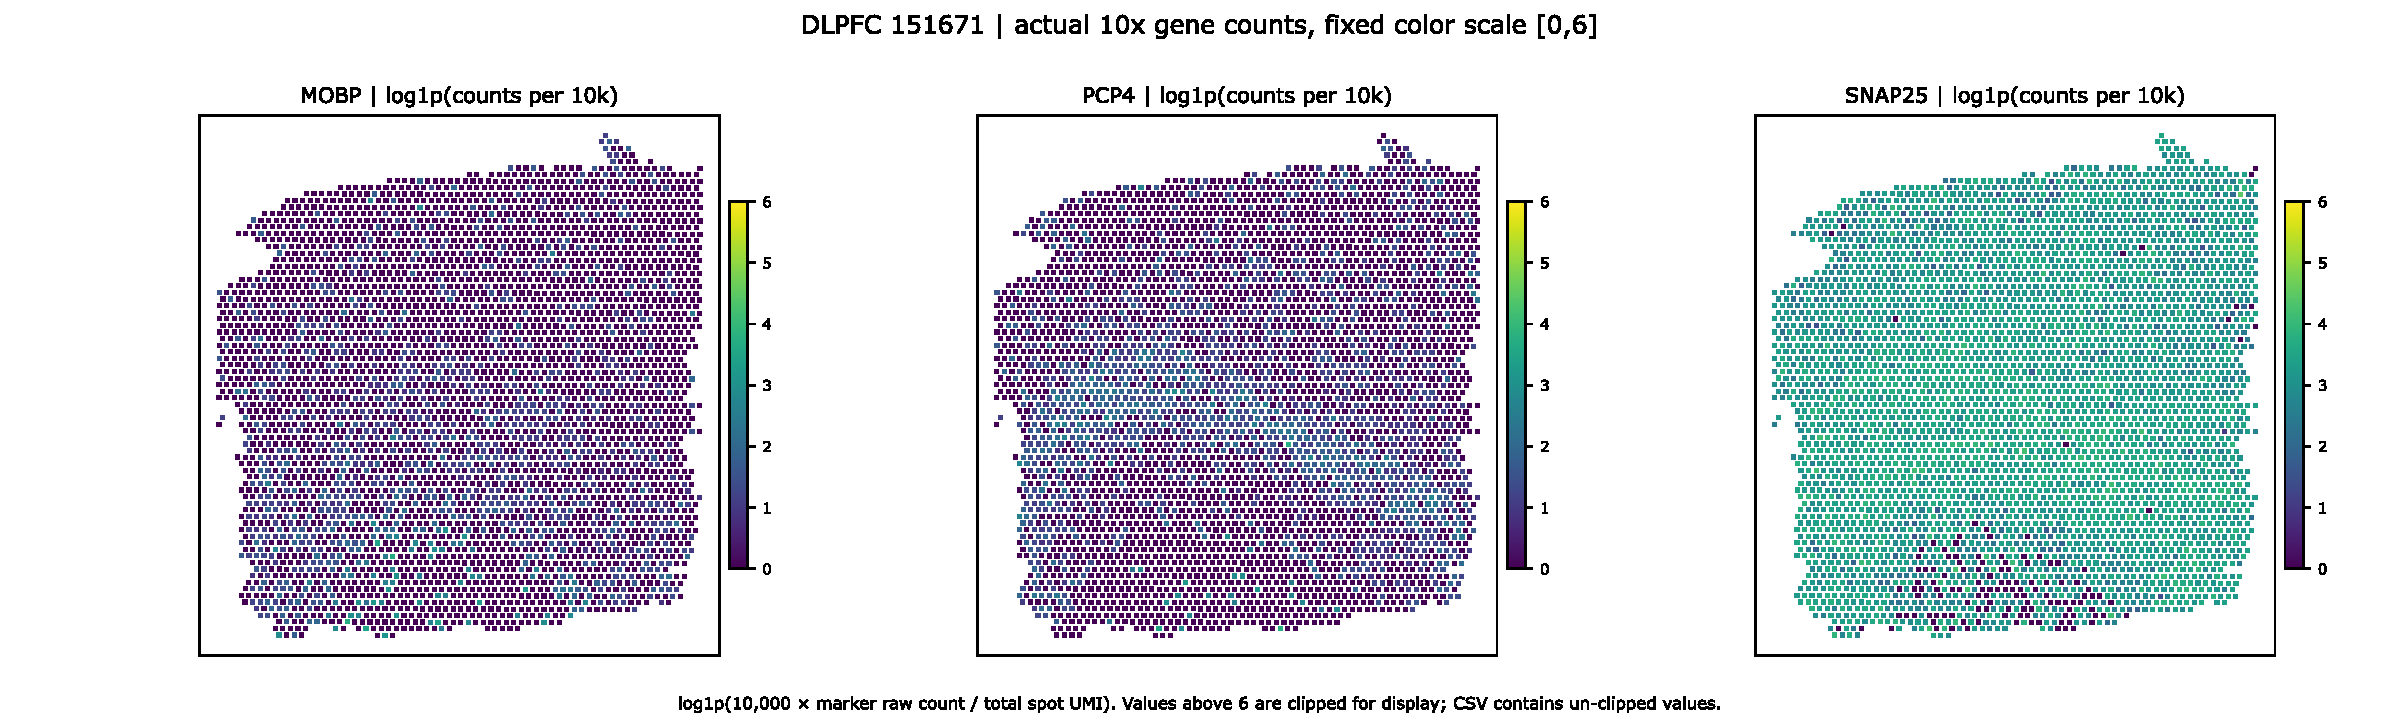
\includegraphics[width=0.97\linewidth,height=0.72\textheight,keepaspectratio]{E4_SOURCE_FIGURES_20261122_RELEASE/figures_pdf/151671/151671_MOBP_PCP4_SNAP25_expression.pdf}
\captionof{figure}{DLPFC切片151671：MOBP/PCP4/SNAP25表达三联图（原始E4图件转换的矢量PDF；聚类编号未根据参考标签重排）。}
\label{fig:cc-e4-app-151671-markers}
\end{minipage}\par\medskip
}{%
\par\noindent\emph{[编译提示：未找到该图件的PDF，请检查相对路径。]}\par
}
\IfFileExists{E4_SOURCE_FIGURES_20261122_RELEASE/figures_pdf/151671/151671_reference_A_B_confusion.pdf}{%
\par\noindent\begin{minipage}{\linewidth}
\centering
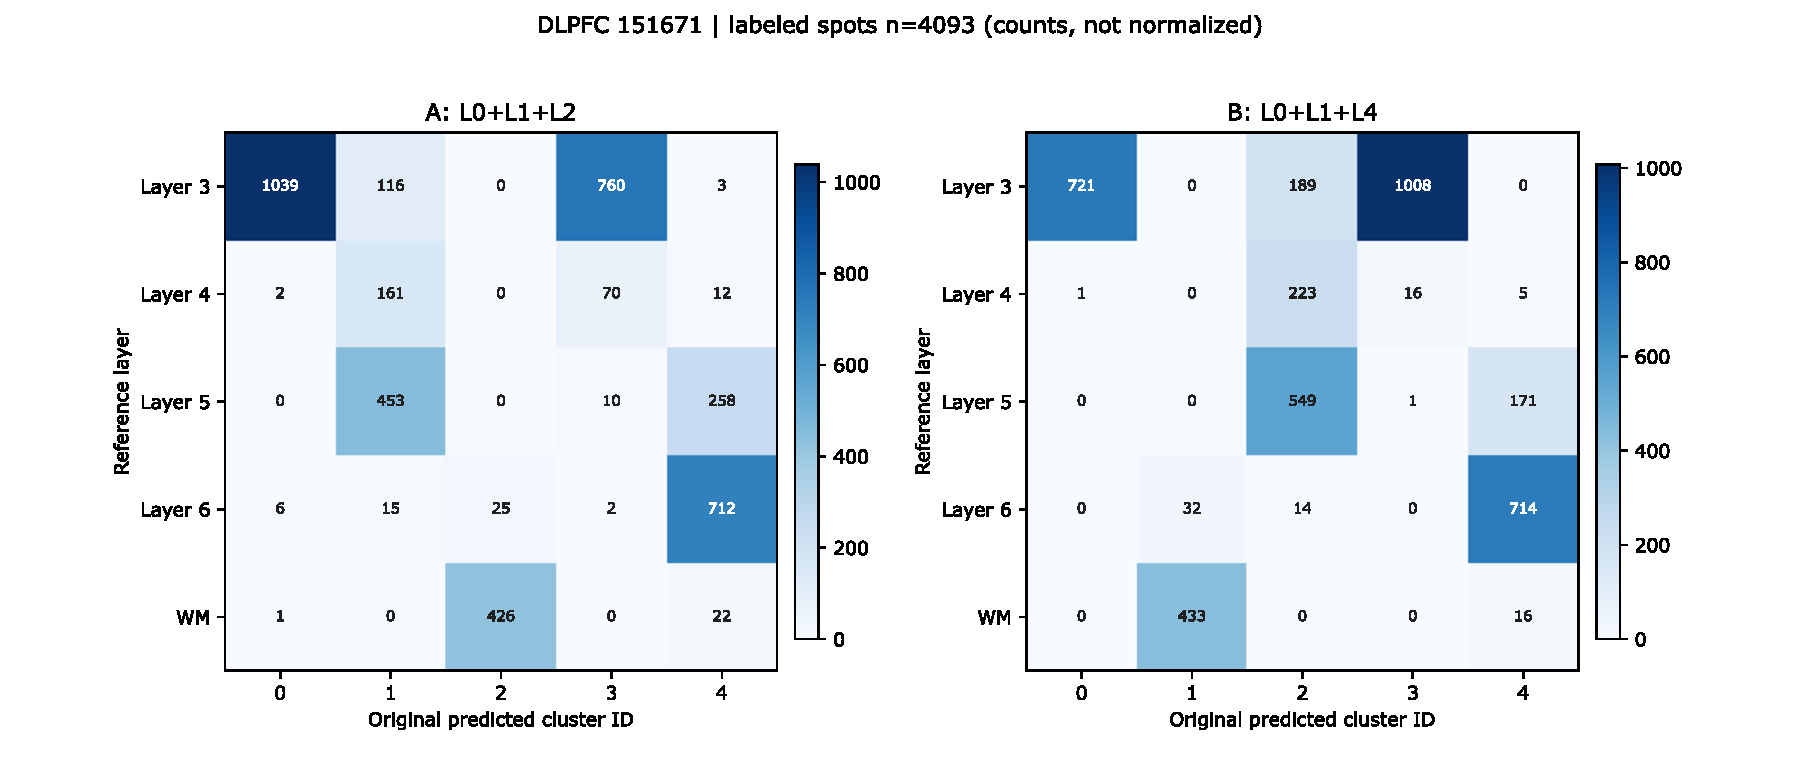
\includegraphics[width=0.97\linewidth,height=0.72\textheight,keepaspectratio]{E4_SOURCE_FIGURES_20261122_RELEASE/figures_pdf/151671/151671_reference_A_B_confusion.pdf}
\captionof{figure}{DLPFC切片151671：参考层与A/B簇交叉计数图（原始E4图件转换的矢量PDF；聚类编号未根据参考标签重排）。}
\label{fig:cc-e4-app-151671-confusion}
\end{minipage}\par\medskip
}{%
\par\noindent\emph{[编译提示：未找到该图件的PDF，请检查相对路径。]}\par
}
\subsection{DLPFC切片151672}
\IfFileExists{E4_SOURCE_FIGURES_20261122_RELEASE/figures_pdf/151672/151672_reference_A_B_spatial.pdf}{%
\par\noindent\begin{minipage}{\linewidth}
\centering
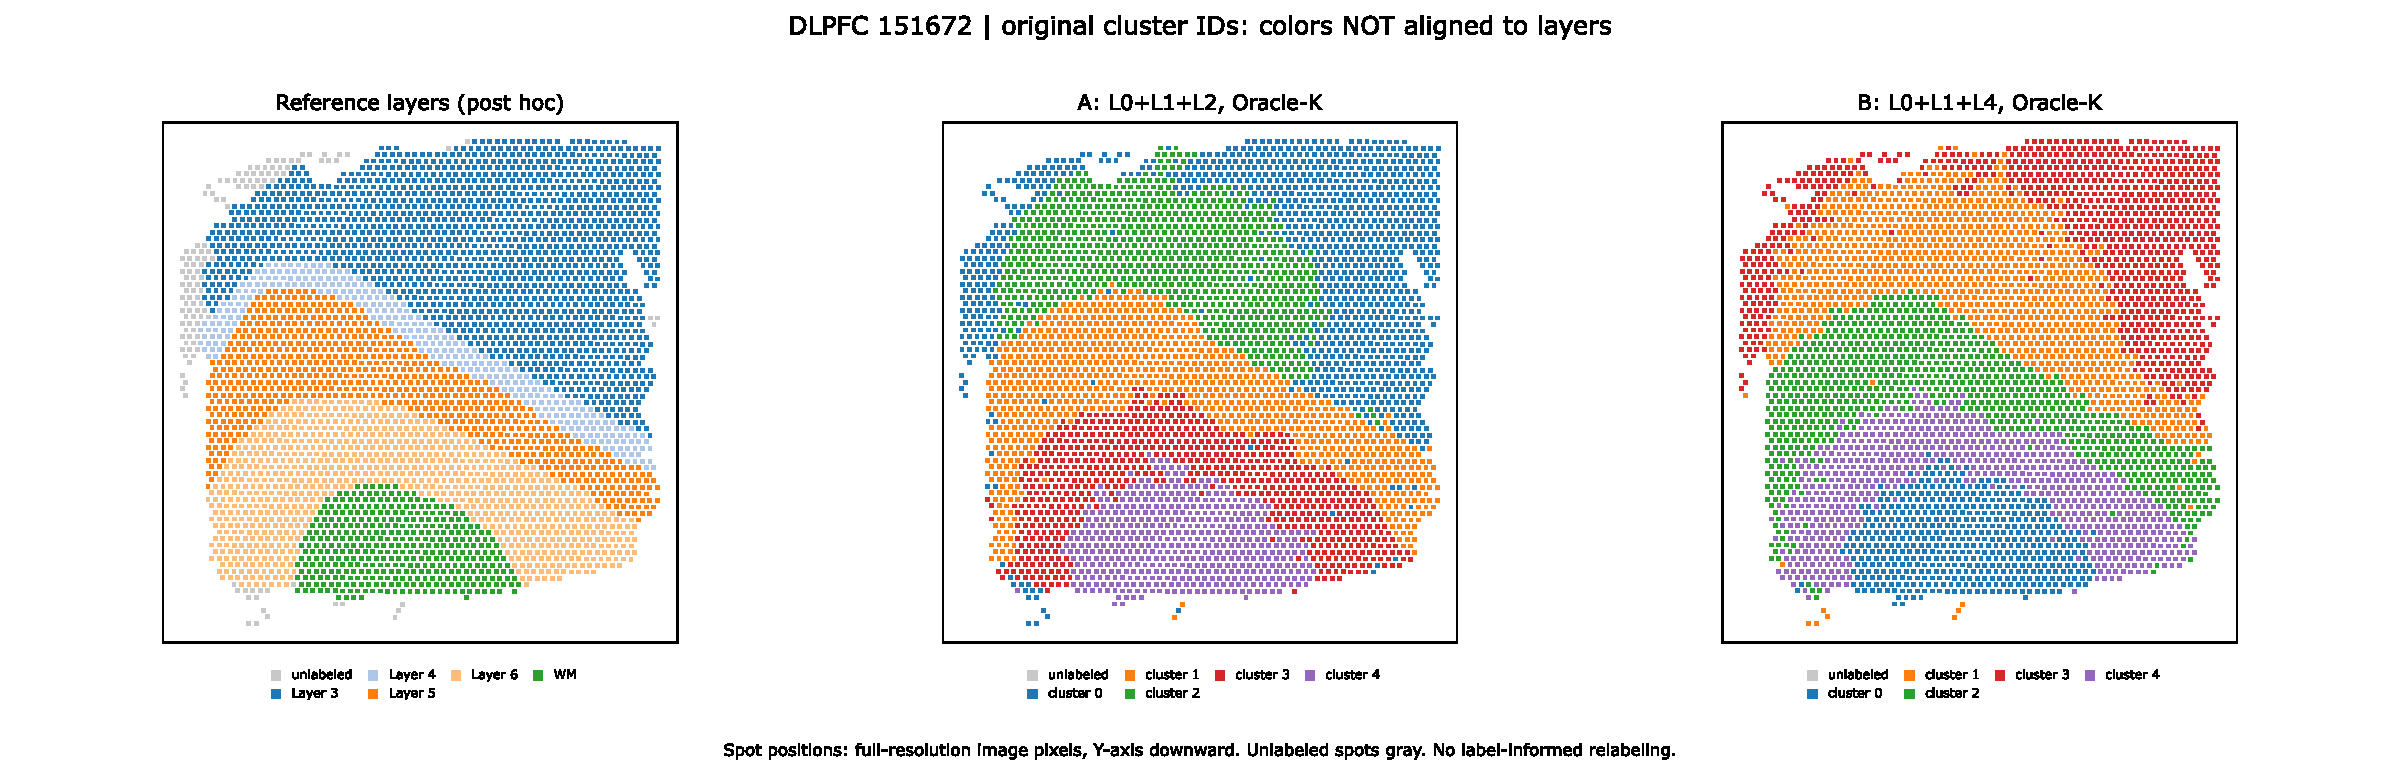
\includegraphics[width=0.97\linewidth,height=0.72\textheight,keepaspectratio]{E4_SOURCE_FIGURES_20261122_RELEASE/figures_pdf/151672/151672_reference_A_B_spatial.pdf}
\captionof{figure}{DLPFC切片151672：参考层与A/B原始聚类三联图（原始E4图件转换的矢量PDF；聚类编号未根据参考标签重排）。}
\label{fig:cc-e4-app-151672-map}
\end{minipage}\par\medskip
}{%
\par\noindent\emph{[编译提示：未找到该图件的PDF，请检查相对路径。]}\par
}
\IfFileExists{E4_SOURCE_FIGURES_20261122_RELEASE/figures_pdf/151672/151672_MOBP_PCP4_SNAP25_expression.pdf}{%
\par\noindent\begin{minipage}{\linewidth}
\centering
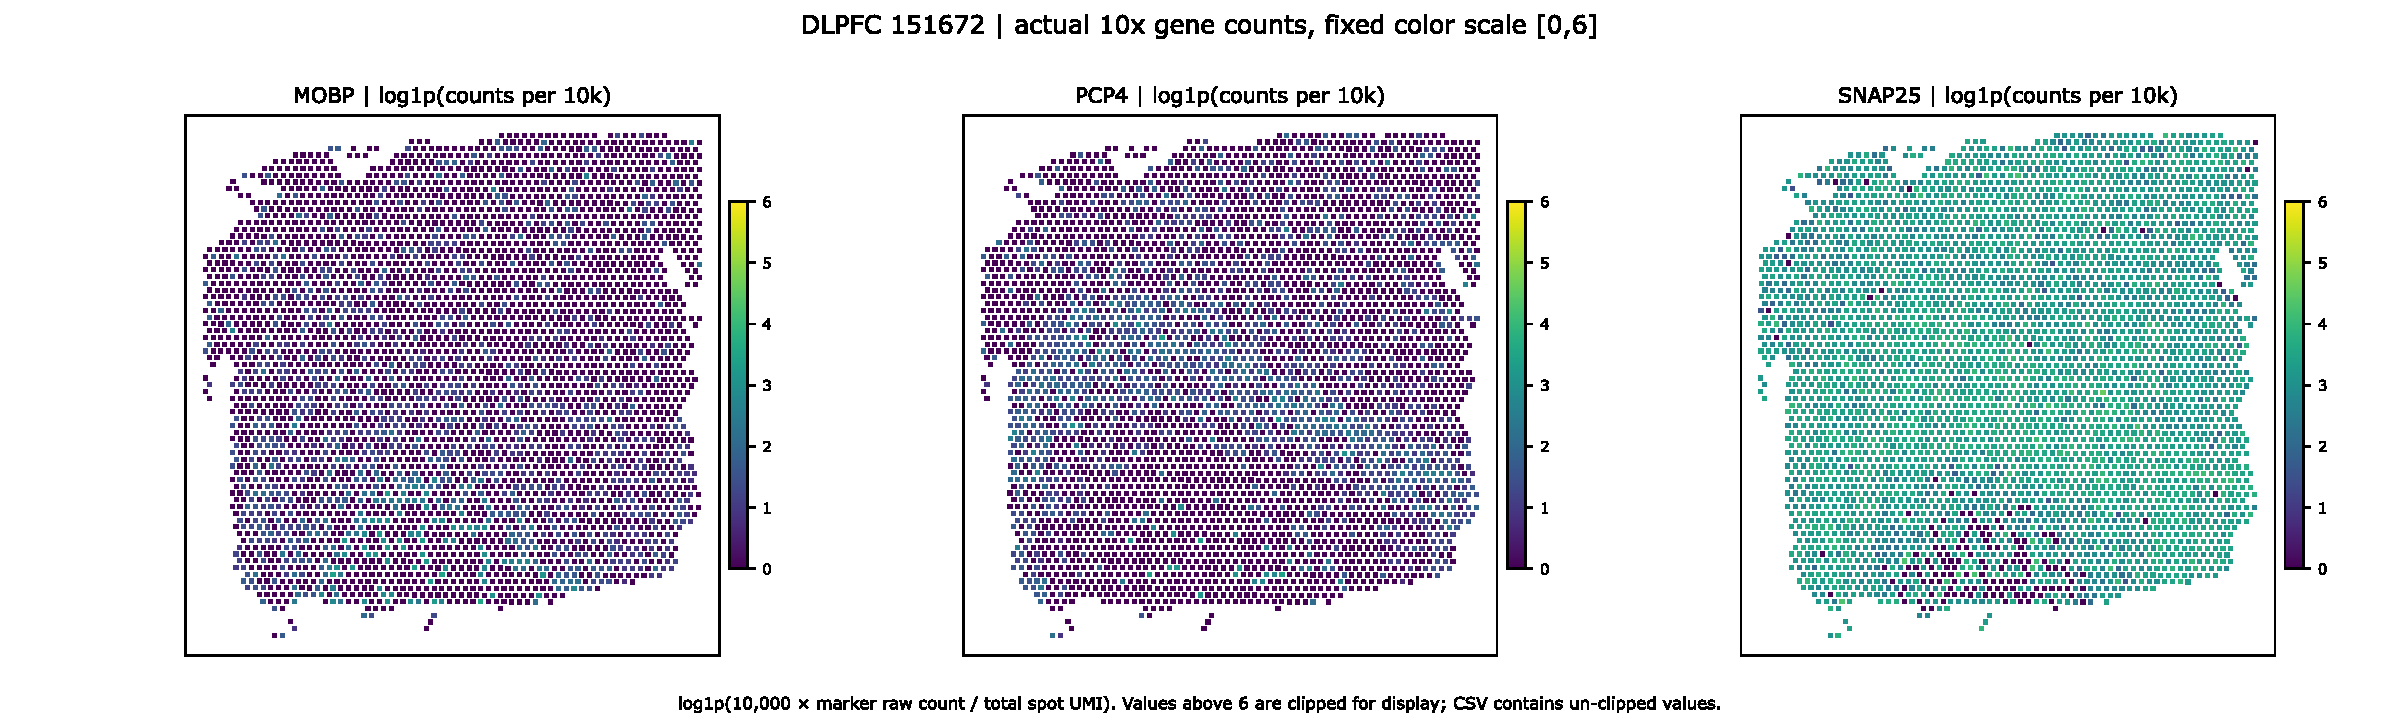
\includegraphics[width=0.97\linewidth,height=0.72\textheight,keepaspectratio]{E4_SOURCE_FIGURES_20261122_RELEASE/figures_pdf/151672/151672_MOBP_PCP4_SNAP25_expression.pdf}
\captionof{figure}{DLPFC切片151672：MOBP/PCP4/SNAP25表达三联图（原始E4图件转换的矢量PDF；聚类编号未根据参考标签重排）。}
\label{fig:cc-e4-app-151672-markers}
\end{minipage}\par\medskip
}{%
\par\noindent\emph{[编译提示：未找到该图件的PDF，请检查相对路径。]}\par
}
\IfFileExists{E4_SOURCE_FIGURES_20261122_RELEASE/figures_pdf/151672/151672_reference_A_B_confusion.pdf}{%
\par\noindent\begin{minipage}{\linewidth}
\centering
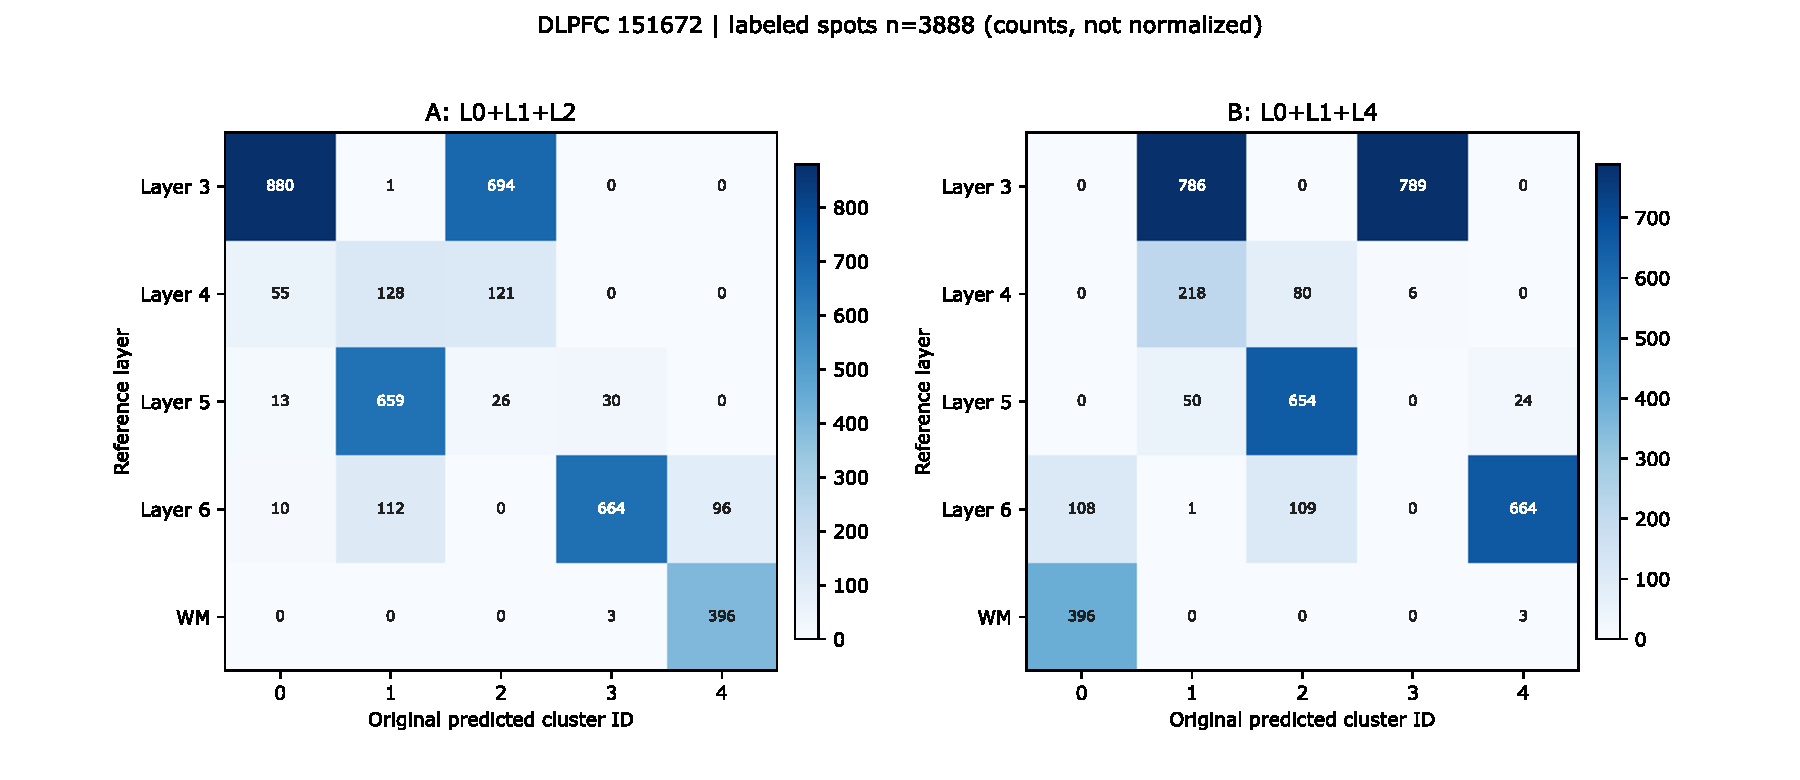
\includegraphics[width=0.97\linewidth,height=0.72\textheight,keepaspectratio]{E4_SOURCE_FIGURES_20261122_RELEASE/figures_pdf/151672/151672_reference_A_B_confusion.pdf}
\captionof{figure}{DLPFC切片151672：参考层与A/B簇交叉计数图（原始E4图件转换的矢量PDF；聚类编号未根据参考标签重排）。}
\label{fig:cc-e4-app-151672-confusion}
\end{minipage}\par\medskip
}{%
\par\noindent\emph{[编译提示：未找到该图件的PDF，请检查相对路径。]}\par
}
\subsection{DLPFC切片151673}
\IfFileExists{E4_SOURCE_FIGURES_20261122_RELEASE/figures_pdf/151673/151673_reference_A_B_spatial.pdf}{%
\par\noindent\begin{minipage}{\linewidth}
\centering
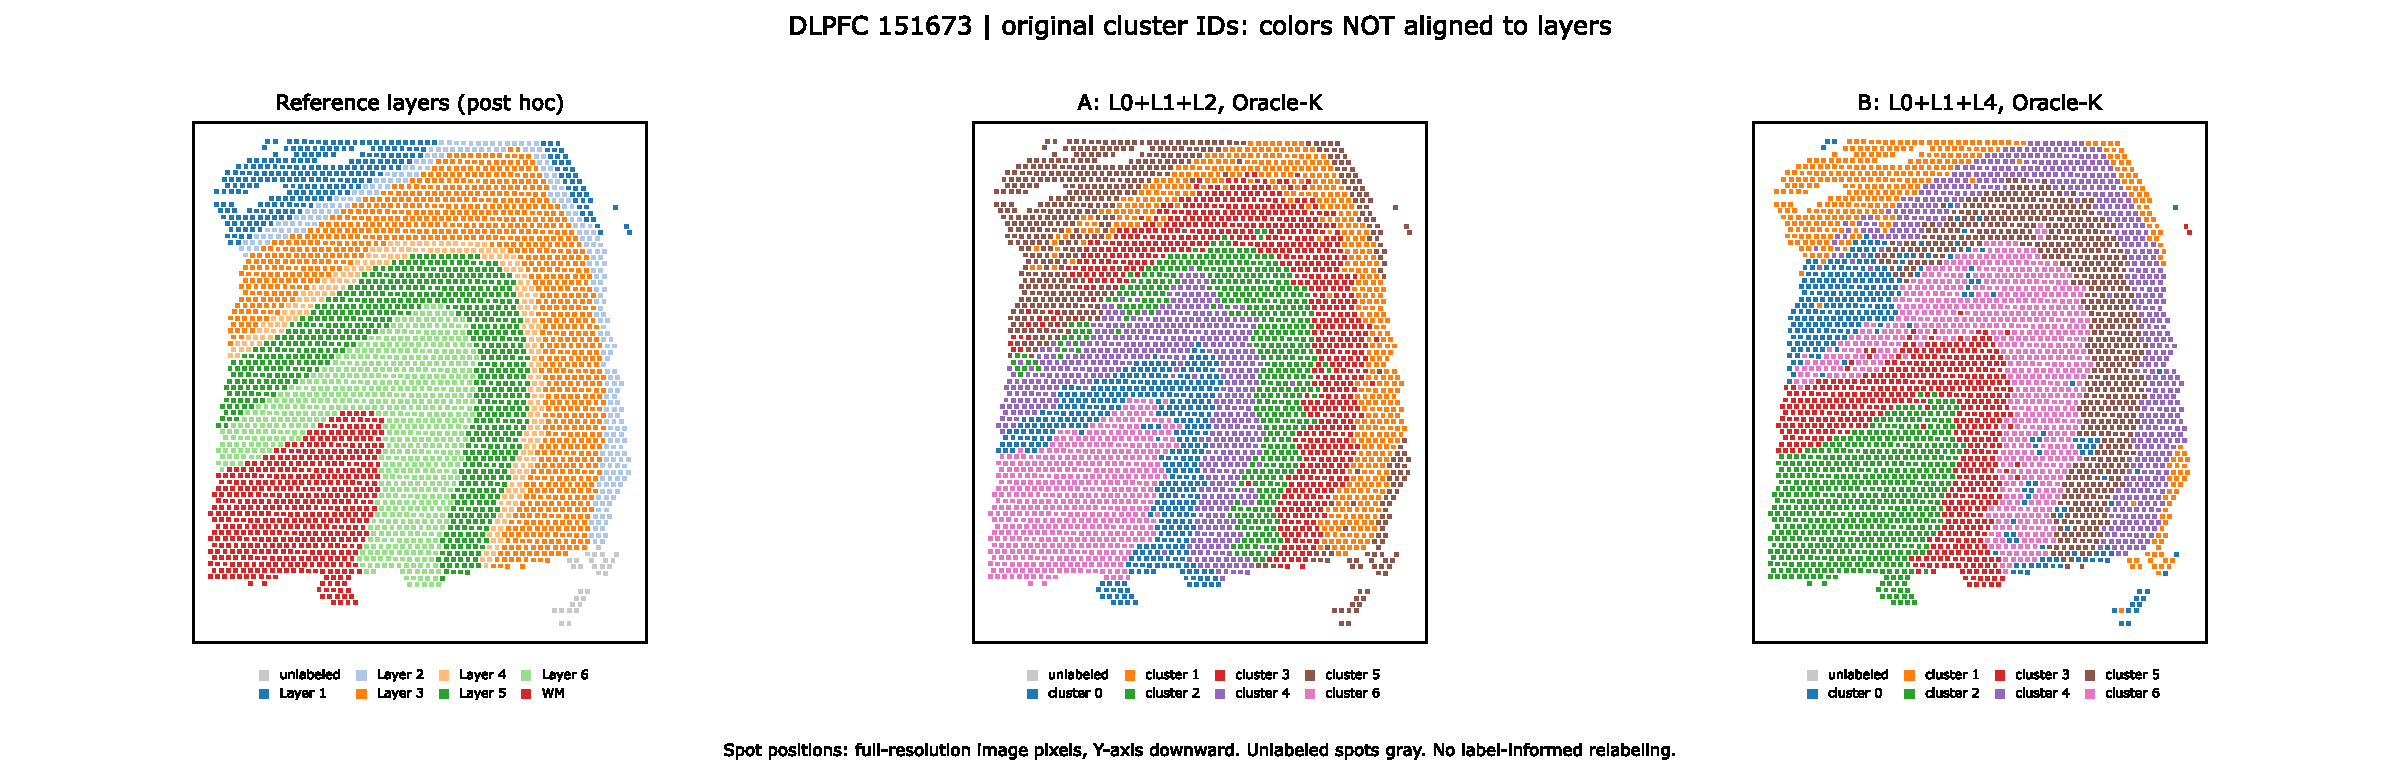
\includegraphics[width=0.97\linewidth,height=0.72\textheight,keepaspectratio]{E4_SOURCE_FIGURES_20261122_RELEASE/figures_pdf/151673/151673_reference_A_B_spatial.pdf}
\captionof{figure}{DLPFC切片151673：参考层与A/B原始聚类三联图（原始E4图件转换的矢量PDF；聚类编号未根据参考标签重排）。}
\label{fig:cc-e4-app-151673-map}
\end{minipage}\par\medskip
}{%
\par\noindent\emph{[编译提示：未找到该图件的PDF，请检查相对路径。]}\par
}
\IfFileExists{E4_SOURCE_FIGURES_20261122_RELEASE/figures_pdf/151673/151673_MOBP_PCP4_SNAP25_expression.pdf}{%
\par\noindent\begin{minipage}{\linewidth}
\centering
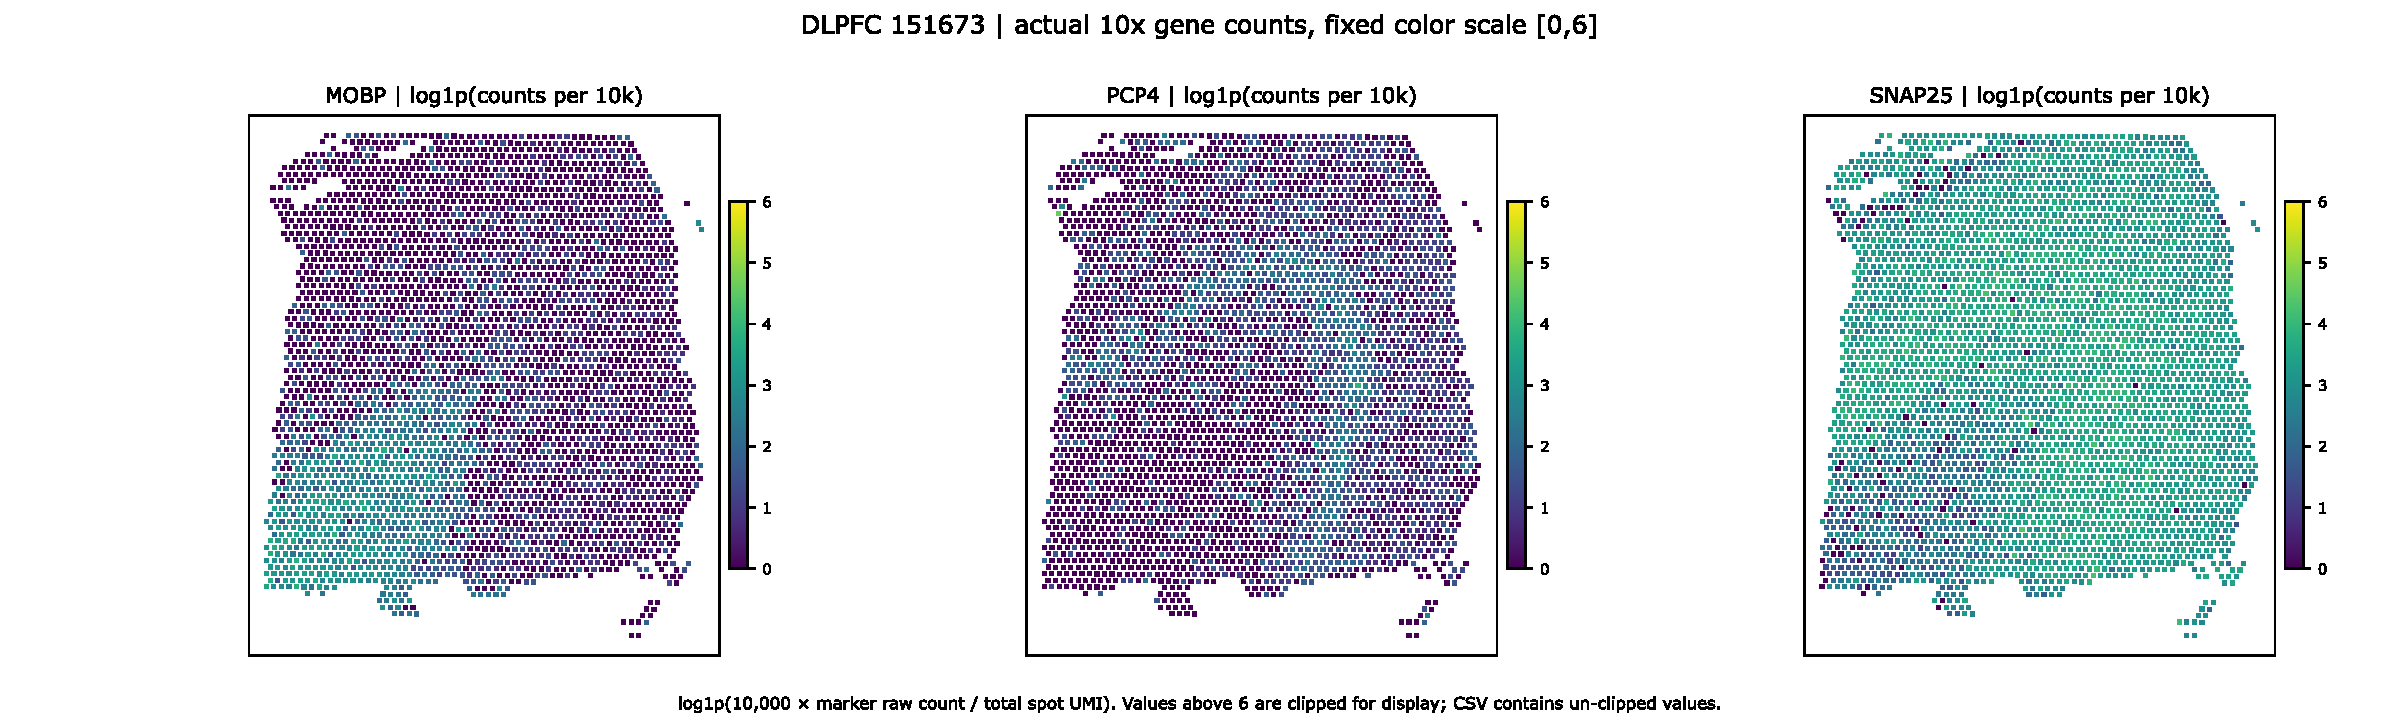
\includegraphics[width=0.97\linewidth,height=0.72\textheight,keepaspectratio]{E4_SOURCE_FIGURES_20261122_RELEASE/figures_pdf/151673/151673_MOBP_PCP4_SNAP25_expression.pdf}
\captionof{figure}{DLPFC切片151673：MOBP/PCP4/SNAP25表达三联图（原始E4图件转换的矢量PDF；聚类编号未根据参考标签重排）。}
\label{fig:cc-e4-app-151673-markers}
\end{minipage}\par\medskip
}{%
\par\noindent\emph{[编译提示：未找到该图件的PDF，请检查相对路径。]}\par
}
\IfFileExists{E4_SOURCE_FIGURES_20261122_RELEASE/figures_pdf/151673/151673_reference_A_B_confusion.pdf}{%
\par\noindent\begin{minipage}{\linewidth}
\centering
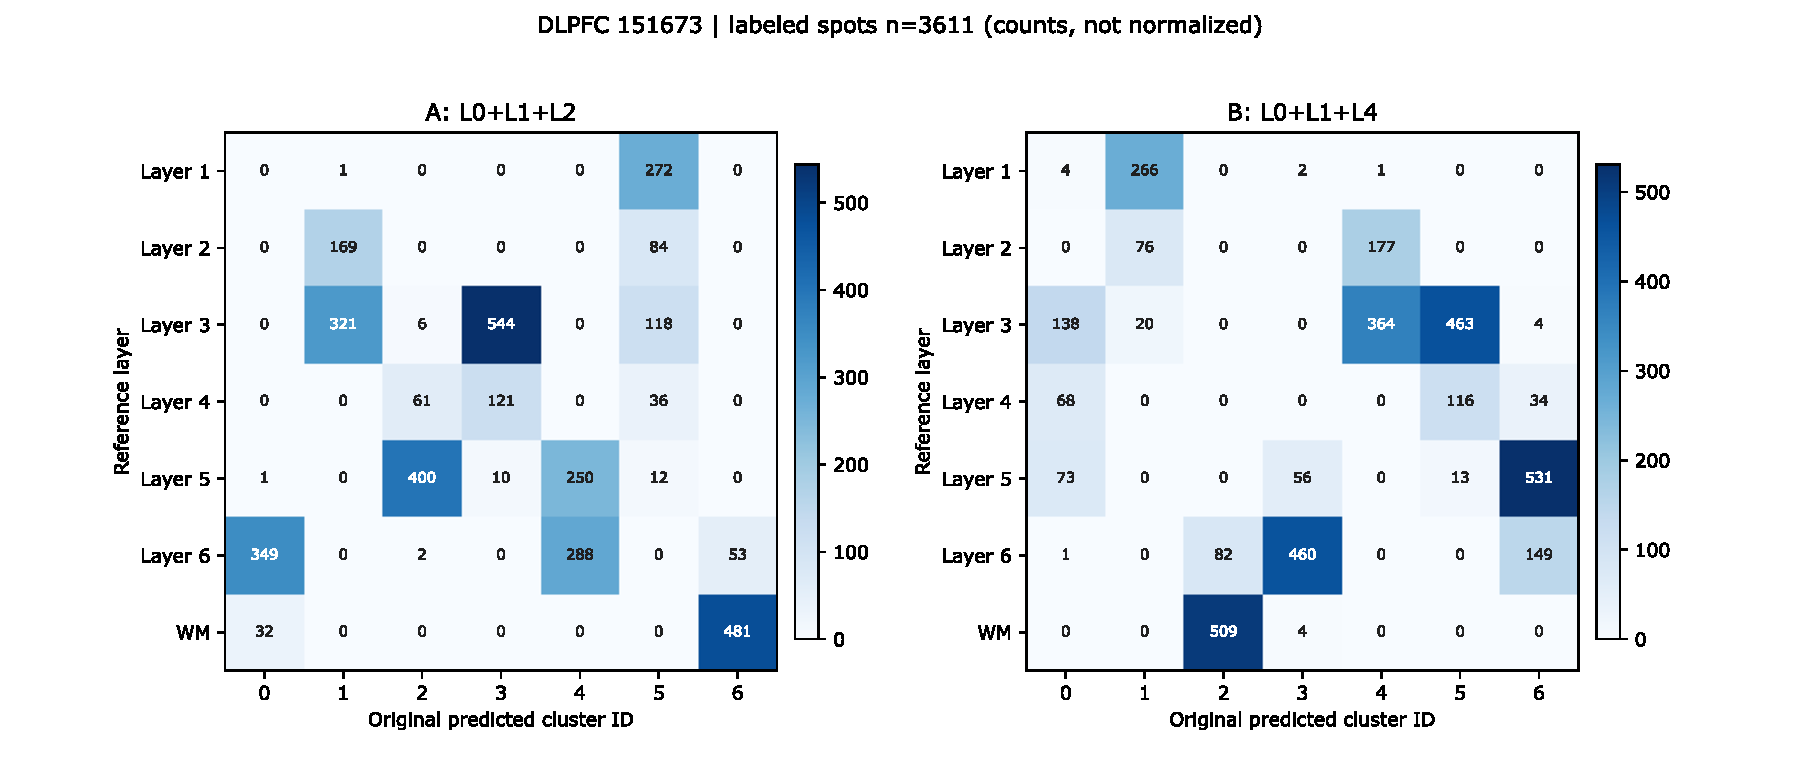
\includegraphics[width=0.97\linewidth,height=0.72\textheight,keepaspectratio]{E4_SOURCE_FIGURES_20261122_RELEASE/figures_pdf/151673/151673_reference_A_B_confusion.pdf}
\captionof{figure}{DLPFC切片151673：参考层与A/B簇交叉计数图（原始E4图件转换的矢量PDF；聚类编号未根据参考标签重排）。}
\label{fig:cc-e4-app-151673-confusion}
\end{minipage}\par\medskip
}{%
\par\noindent\emph{[编译提示：未找到该图件的PDF，请检查相对路径。]}\par
}
\subsection{DLPFC切片151674}
\IfFileExists{E4_SOURCE_FIGURES_20261122_RELEASE/figures_pdf/151674/151674_reference_A_B_spatial.pdf}{%
\par\noindent\begin{minipage}{\linewidth}
\centering
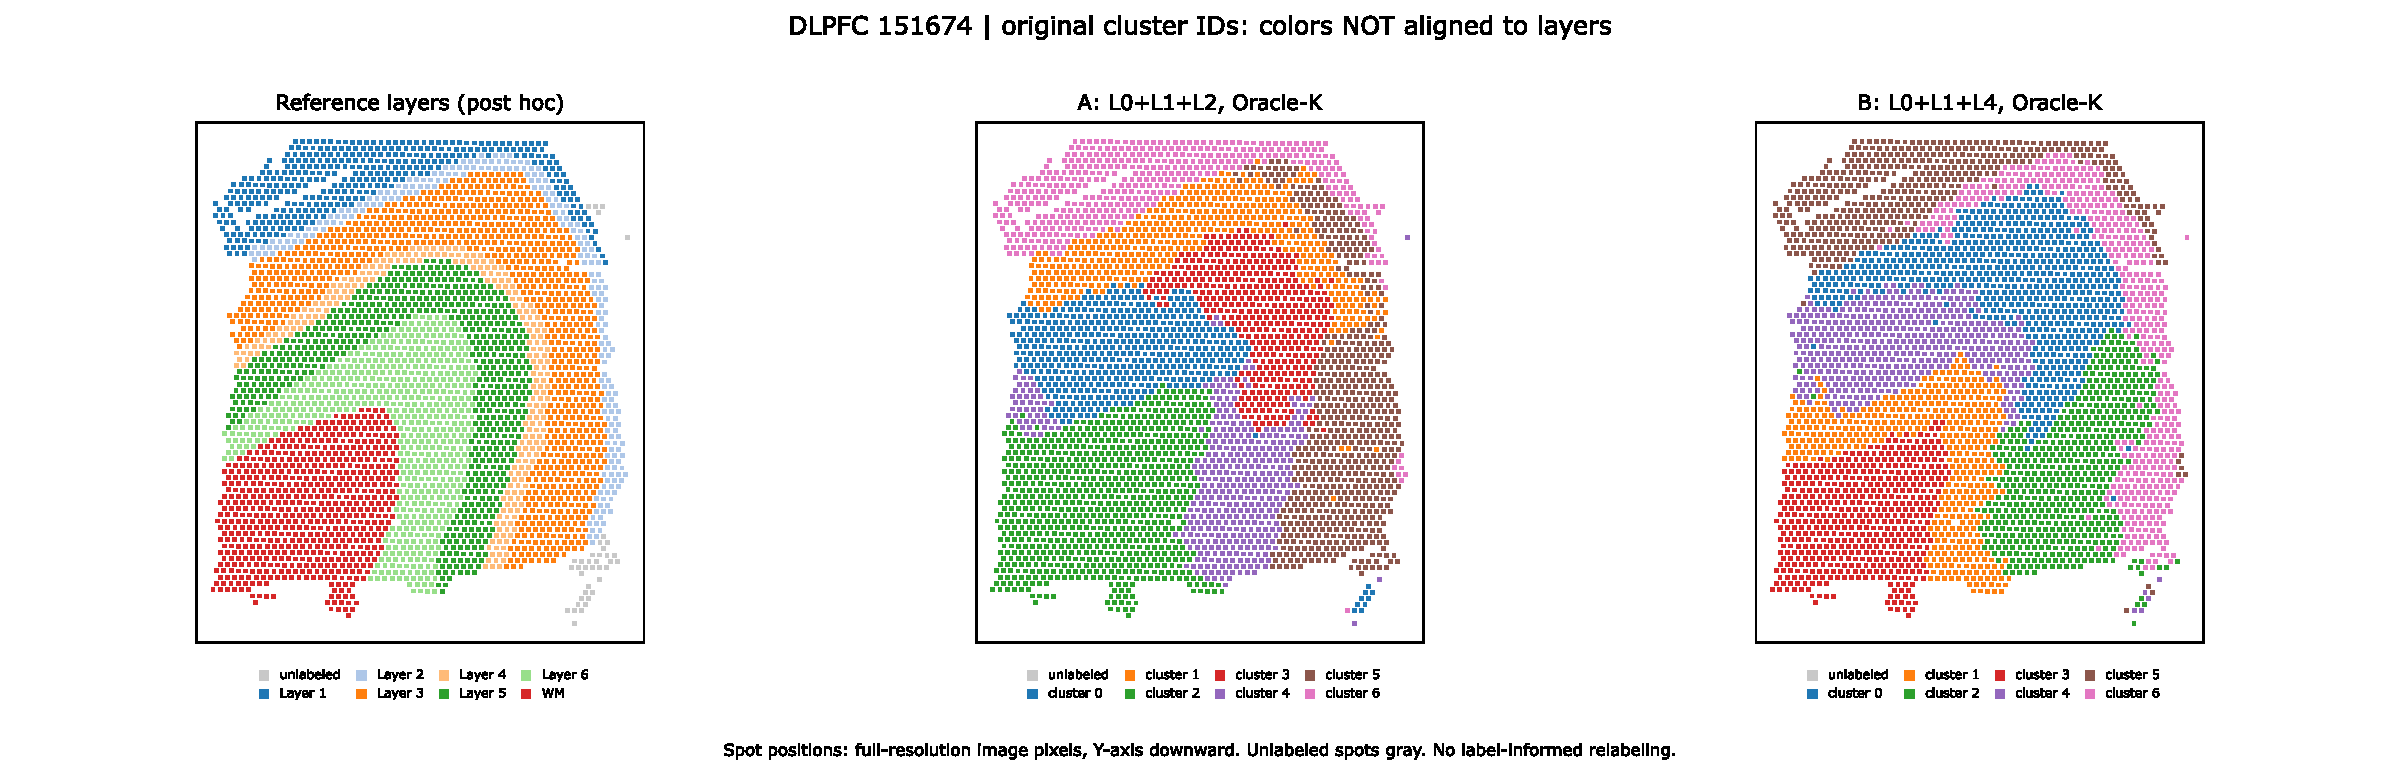
\includegraphics[width=0.97\linewidth,height=0.72\textheight,keepaspectratio]{E4_SOURCE_FIGURES_20261122_RELEASE/figures_pdf/151674/151674_reference_A_B_spatial.pdf}
\captionof{figure}{DLPFC切片151674：参考层与A/B原始聚类三联图（原始E4图件转换的矢量PDF；聚类编号未根据参考标签重排）。}
\label{fig:cc-e4-app-151674-map}
\end{minipage}\par\medskip
}{%
\par\noindent\emph{[编译提示：未找到该图件的PDF，请检查相对路径。]}\par
}
\IfFileExists{E4_SOURCE_FIGURES_20261122_RELEASE/figures_pdf/151674/151674_MOBP_PCP4_SNAP25_expression.pdf}{%
\par\noindent\begin{minipage}{\linewidth}
\centering
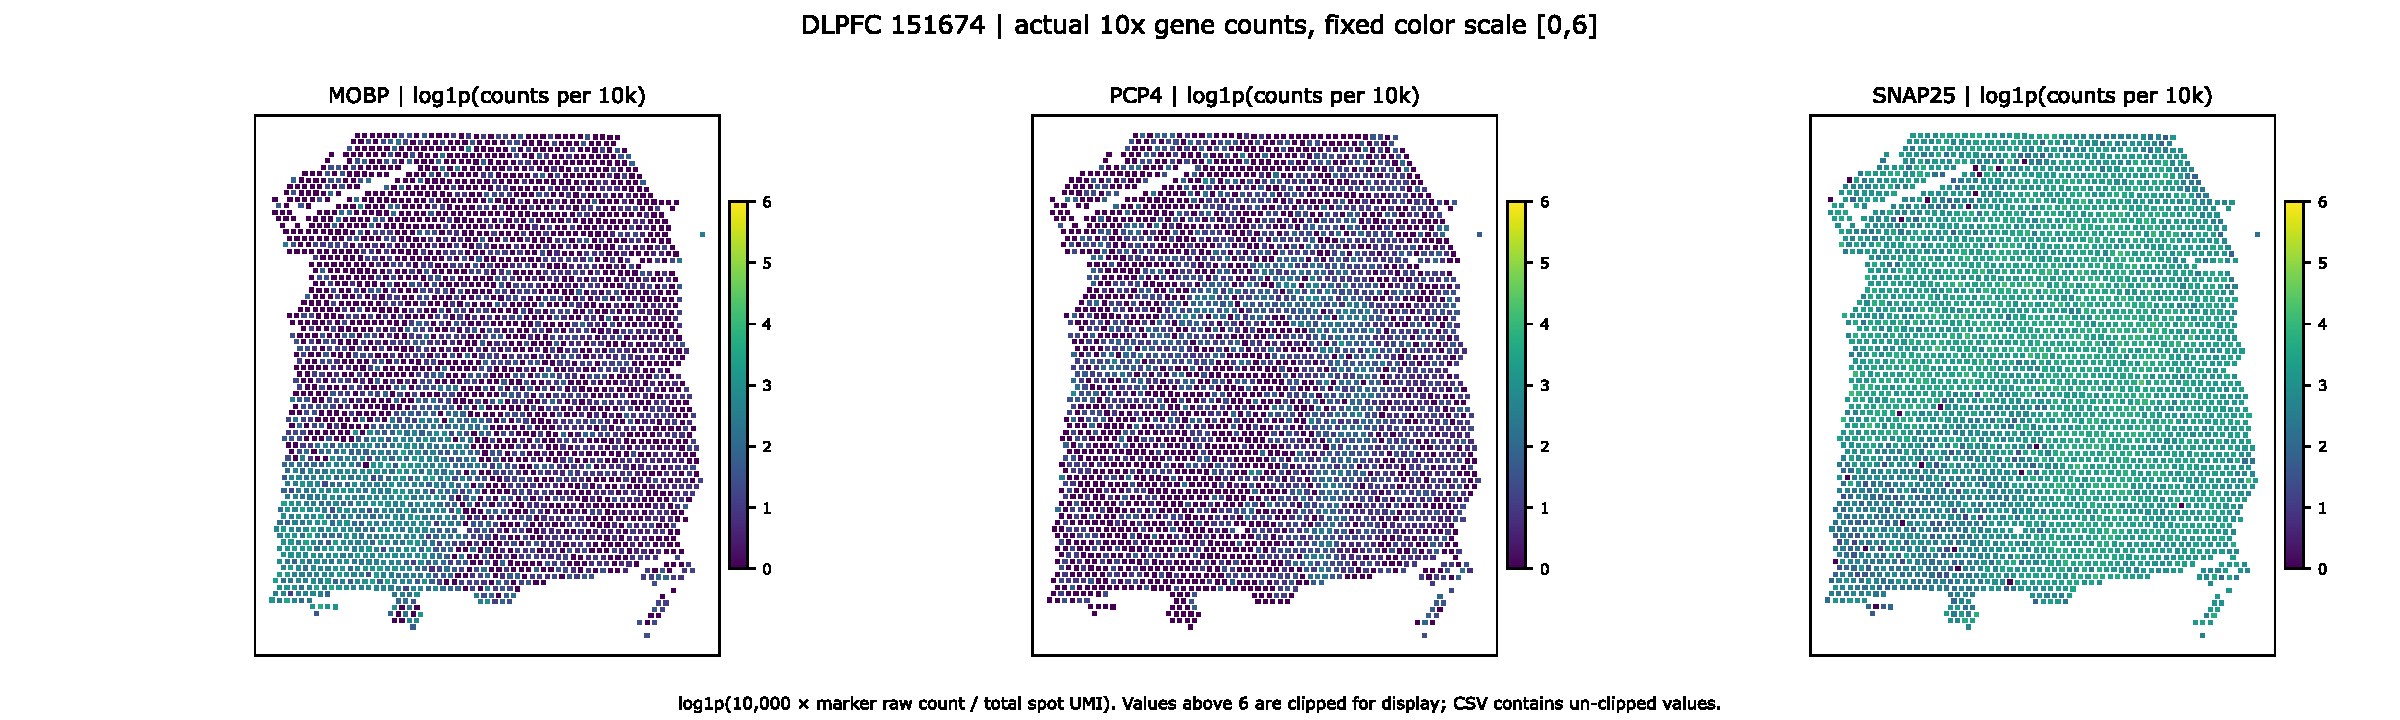
\includegraphics[width=0.97\linewidth,height=0.72\textheight,keepaspectratio]{E4_SOURCE_FIGURES_20261122_RELEASE/figures_pdf/151674/151674_MOBP_PCP4_SNAP25_expression.pdf}
\captionof{figure}{DLPFC切片151674：MOBP/PCP4/SNAP25表达三联图（原始E4图件转换的矢量PDF；聚类编号未根据参考标签重排）。}
\label{fig:cc-e4-app-151674-markers}
\end{minipage}\par\medskip
}{%
\par\noindent\emph{[编译提示：未找到该图件的PDF，请检查相对路径。]}\par
}
\IfFileExists{E4_SOURCE_FIGURES_20261122_RELEASE/figures_pdf/151674/151674_reference_A_B_confusion.pdf}{%
\par\noindent\begin{minipage}{\linewidth}
\centering
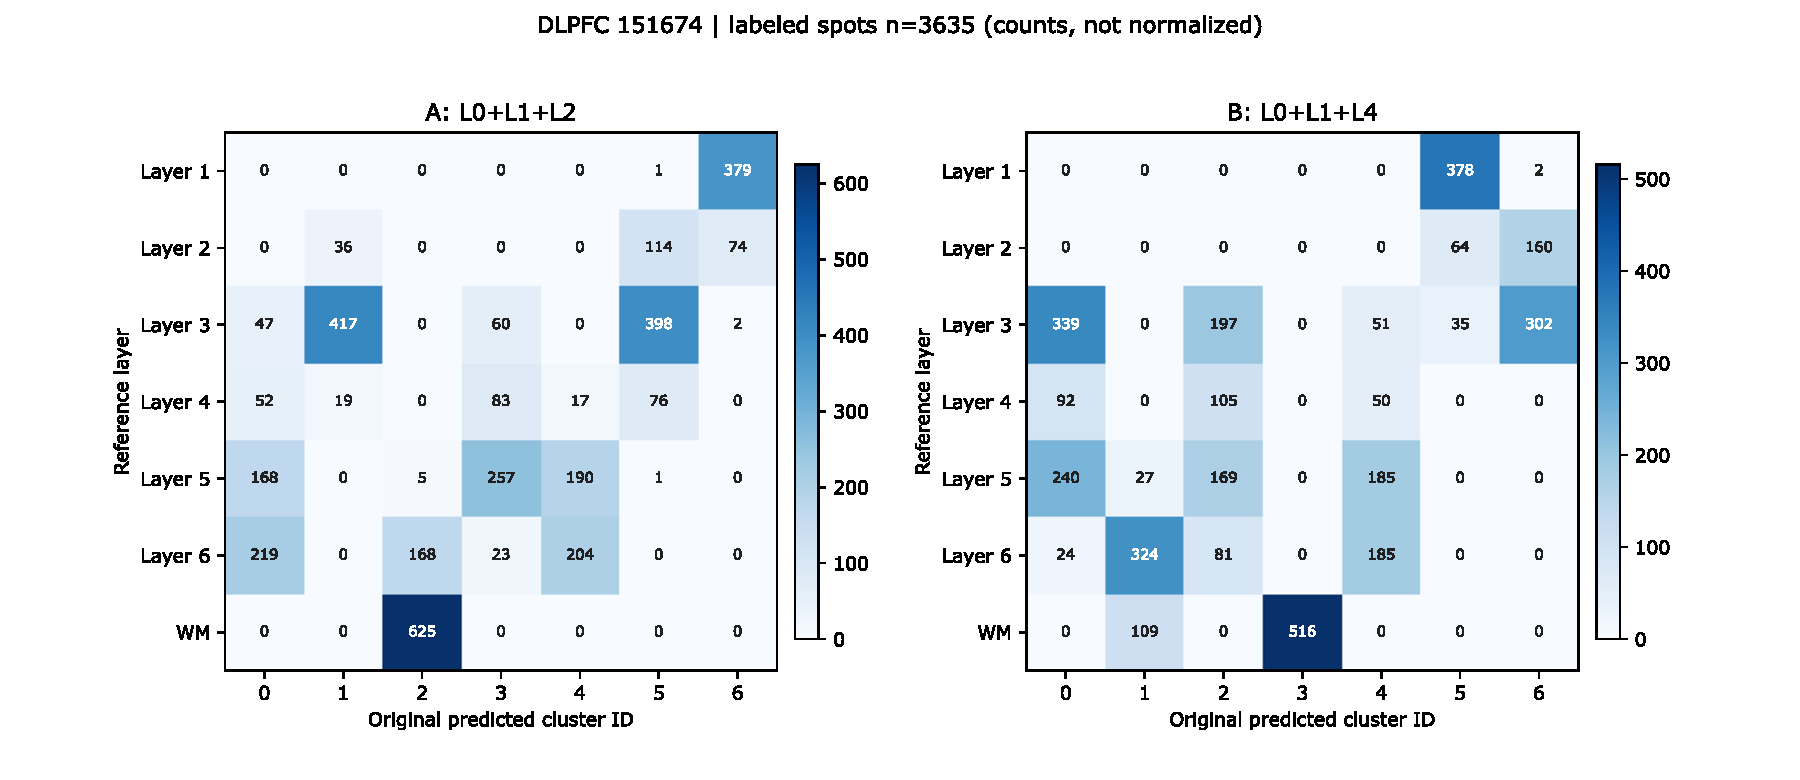
\includegraphics[width=0.97\linewidth,height=0.72\textheight,keepaspectratio]{E4_SOURCE_FIGURES_20261122_RELEASE/figures_pdf/151674/151674_reference_A_B_confusion.pdf}
\captionof{figure}{DLPFC切片151674：参考层与A/B簇交叉计数图（原始E4图件转换的矢量PDF；聚类编号未根据参考标签重排）。}
\label{fig:cc-e4-app-151674-confusion}
\end{minipage}\par\medskip
}{%
\par\noindent\emph{[编译提示：未找到该图件的PDF，请检查相对路径。]}\par
}
\subsection{DLPFC切片151675}
\IfFileExists{E4_SOURCE_FIGURES_20261122_RELEASE/figures_pdf/151675/151675_reference_A_B_spatial.pdf}{%
\par\noindent\begin{minipage}{\linewidth}
\centering
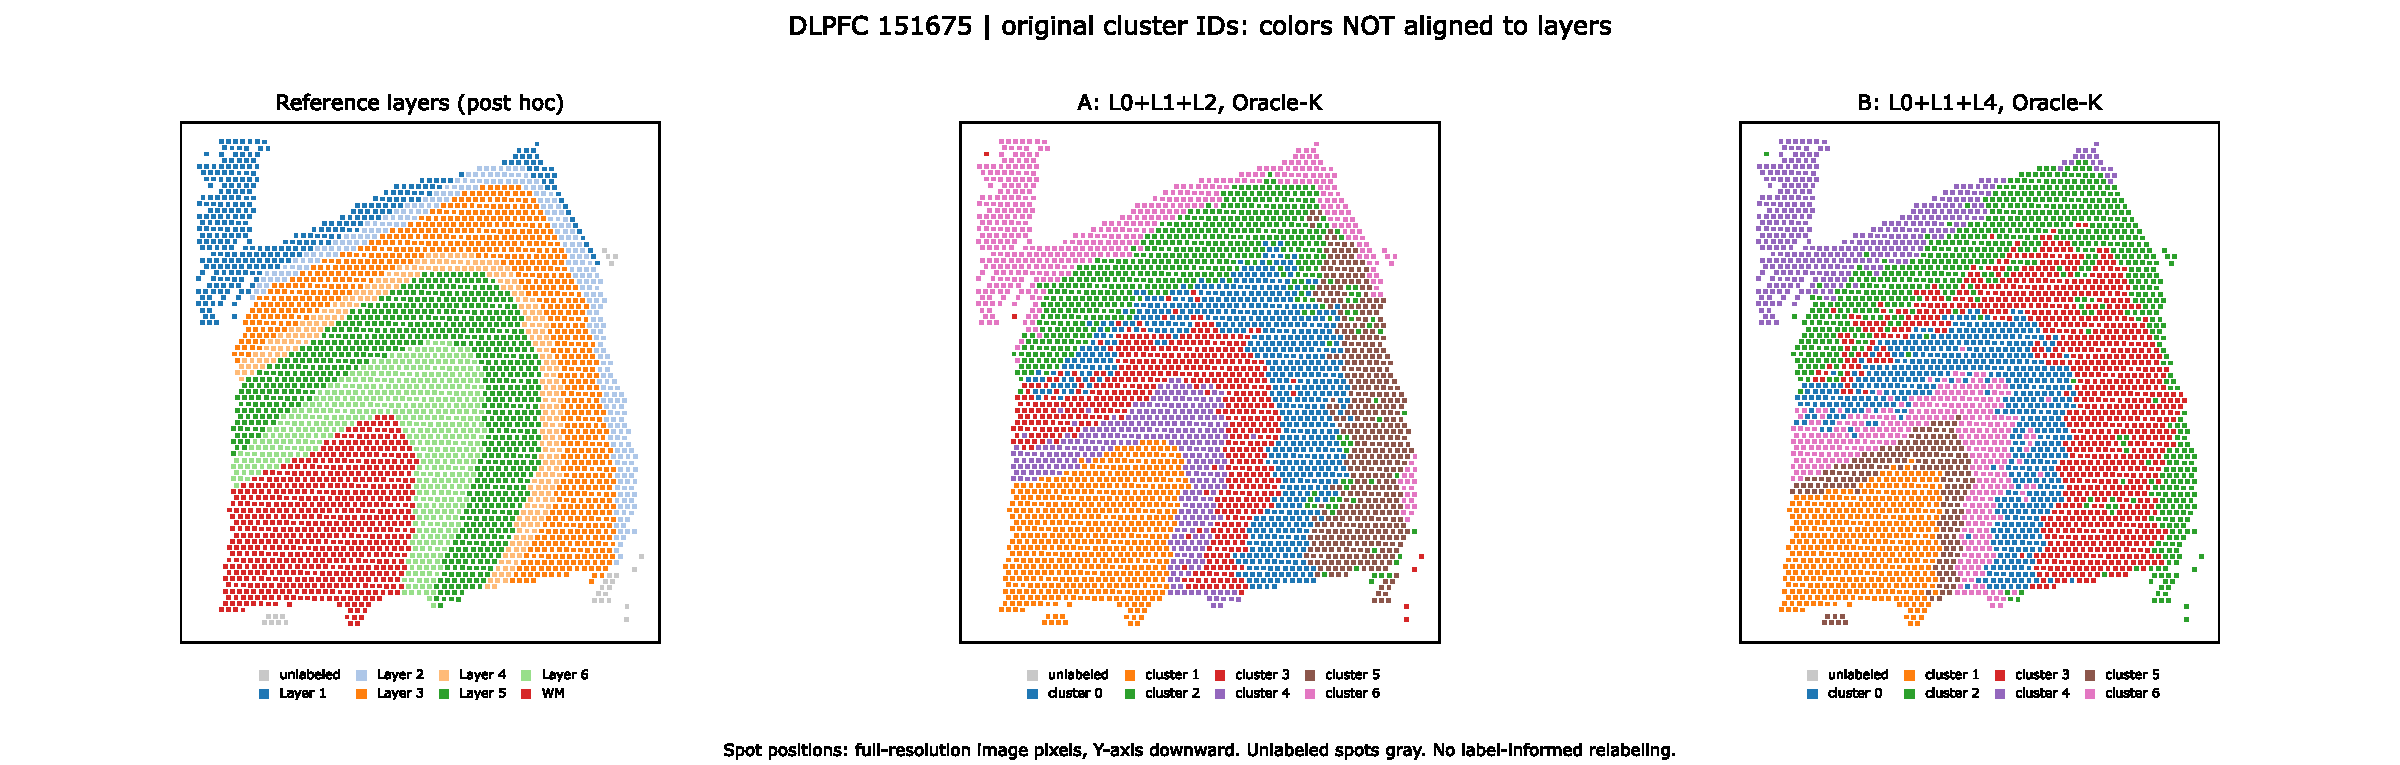
\includegraphics[width=0.97\linewidth,height=0.72\textheight,keepaspectratio]{E4_SOURCE_FIGURES_20261122_RELEASE/figures_pdf/151675/151675_reference_A_B_spatial.pdf}
\captionof{figure}{DLPFC切片151675：参考层与A/B原始聚类三联图（原始E4图件转换的矢量PDF；聚类编号未根据参考标签重排）。}
\label{fig:cc-e4-app-151675-map}
\end{minipage}\par\medskip
}{%
\par\noindent\emph{[编译提示：未找到该图件的PDF，请检查相对路径。]}\par
}
\IfFileExists{E4_SOURCE_FIGURES_20261122_RELEASE/figures_pdf/151675/151675_MOBP_PCP4_SNAP25_expression.pdf}{%
\par\noindent\begin{minipage}{\linewidth}
\centering
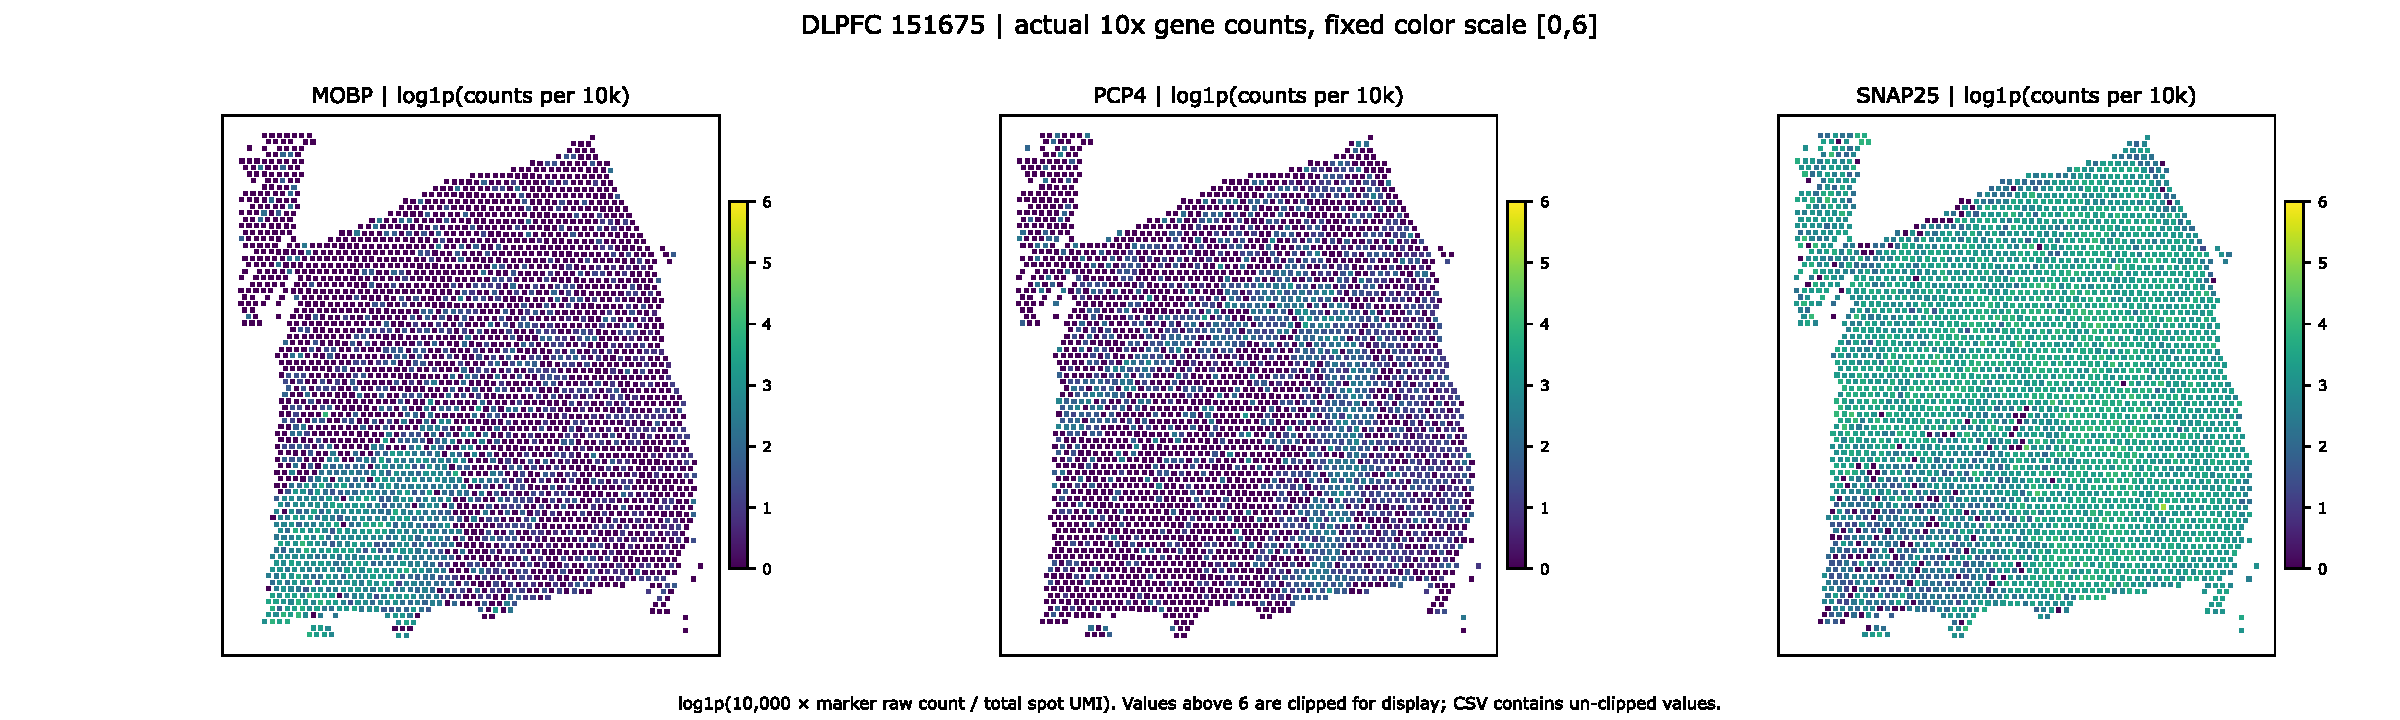
\includegraphics[width=0.97\linewidth,height=0.72\textheight,keepaspectratio]{E4_SOURCE_FIGURES_20261122_RELEASE/figures_pdf/151675/151675_MOBP_PCP4_SNAP25_expression.pdf}
\captionof{figure}{DLPFC切片151675：MOBP/PCP4/SNAP25表达三联图（原始E4图件转换的矢量PDF；聚类编号未根据参考标签重排）。}
\label{fig:cc-e4-app-151675-markers}
\end{minipage}\par\medskip
}{%
\par\noindent\emph{[编译提示：未找到该图件的PDF，请检查相对路径。]}\par
}
\IfFileExists{E4_SOURCE_FIGURES_20261122_RELEASE/figures_pdf/151675/151675_reference_A_B_confusion.pdf}{%
\par\noindent\begin{minipage}{\linewidth}
\centering
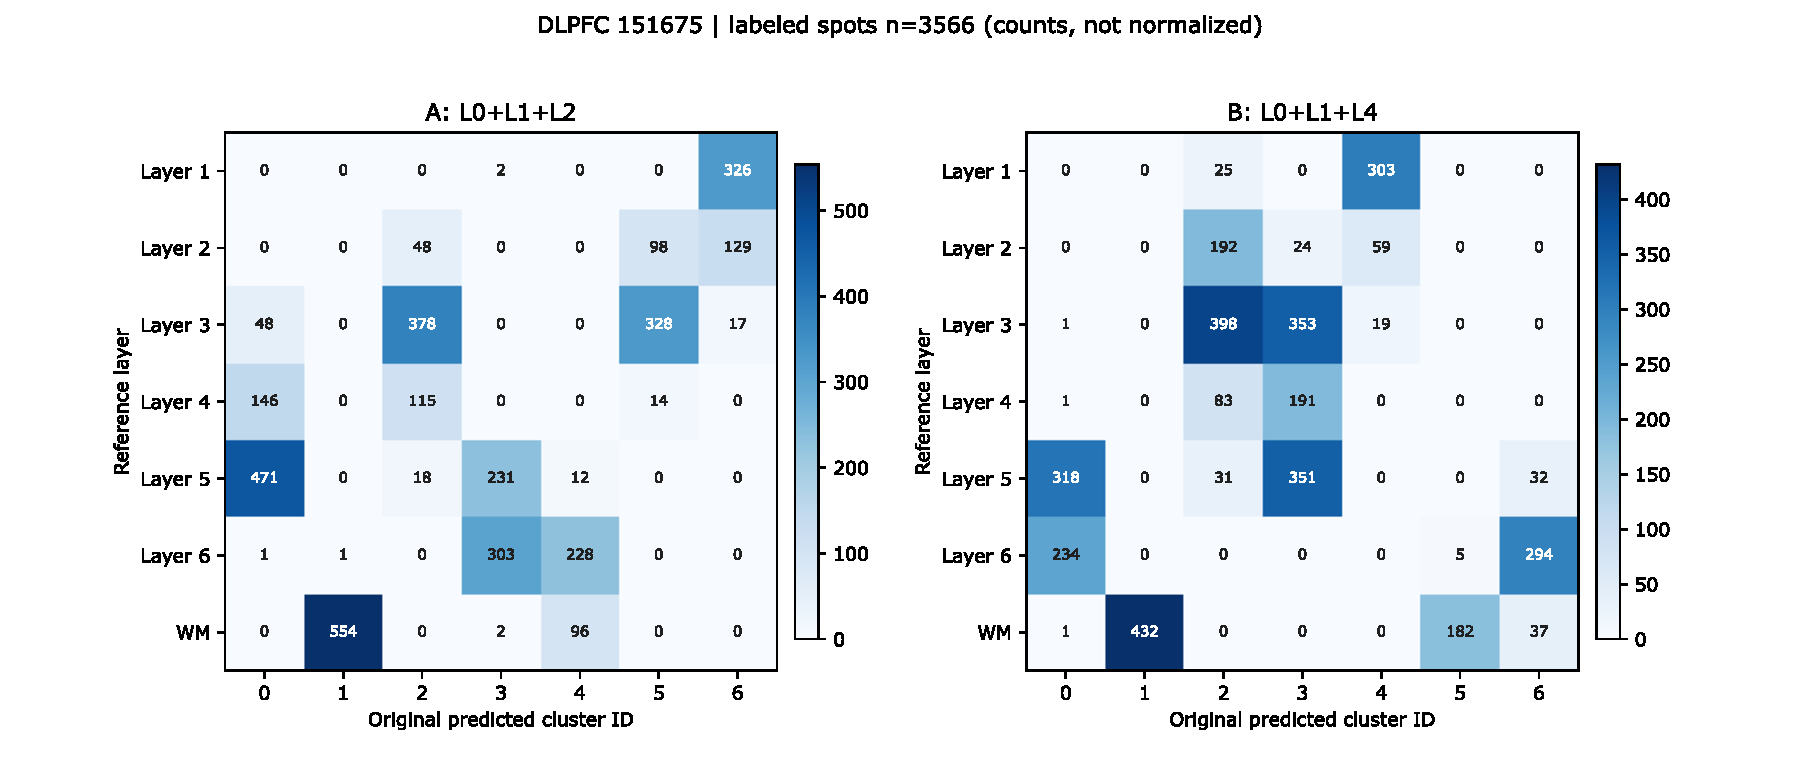
\includegraphics[width=0.97\linewidth,height=0.72\textheight,keepaspectratio]{E4_SOURCE_FIGURES_20261122_RELEASE/figures_pdf/151675/151675_reference_A_B_confusion.pdf}
\captionof{figure}{DLPFC切片151675：参考层与A/B簇交叉计数图（原始E4图件转换的矢量PDF；聚类编号未根据参考标签重排）。}
\label{fig:cc-e4-app-151675-confusion}
\end{minipage}\par\medskip
}{%
\par\noindent\emph{[编译提示：未找到该图件的PDF，请检查相对路径。]}\par
}
\subsection{DLPFC切片151676}
\IfFileExists{E4_SOURCE_FIGURES_20261122_RELEASE/figures_pdf/151676/151676_reference_A_B_spatial.pdf}{%
\par\noindent\begin{minipage}{\linewidth}
\centering
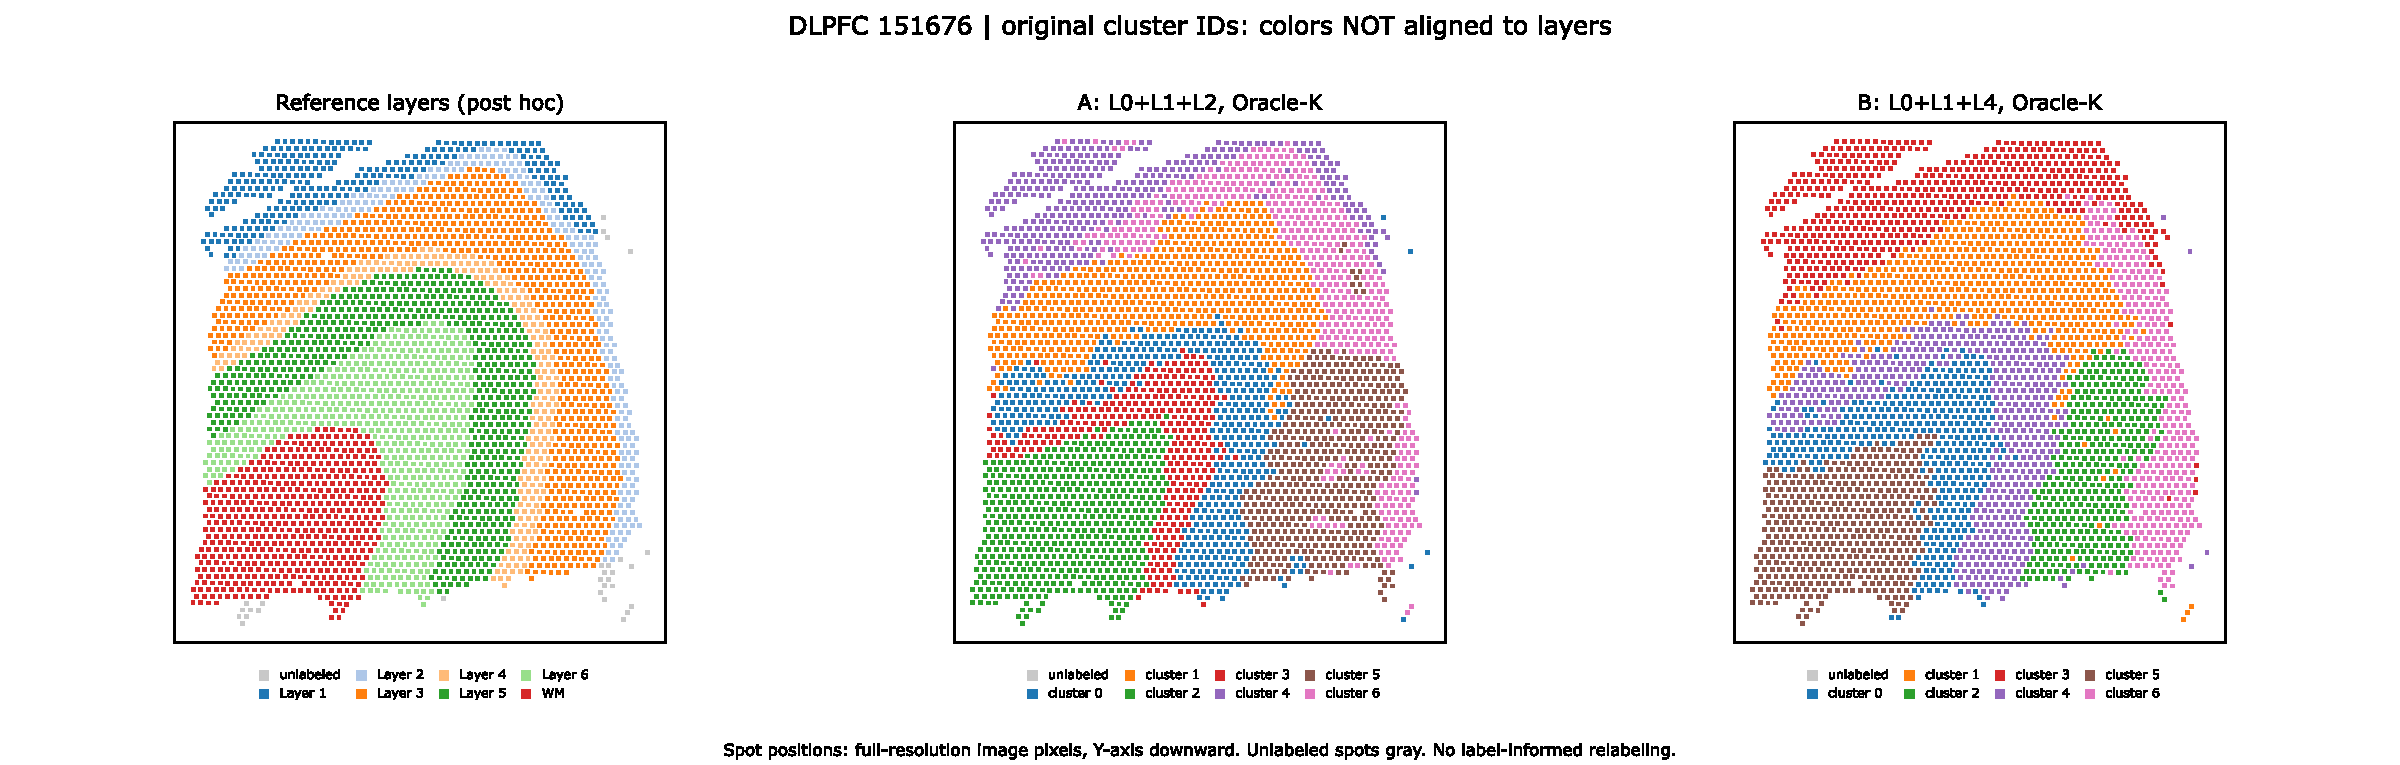
\includegraphics[width=0.97\linewidth,height=0.72\textheight,keepaspectratio]{E4_SOURCE_FIGURES_20261122_RELEASE/figures_pdf/151676/151676_reference_A_B_spatial.pdf}
\captionof{figure}{DLPFC切片151676：参考层与A/B原始聚类三联图（原始E4图件转换的矢量PDF；聚类编号未根据参考标签重排）。}
\label{fig:cc-e4-app-151676-map}
\end{minipage}\par\medskip
}{%
\par\noindent\emph{[编译提示：未找到该图件的PDF，请检查相对路径。]}\par
}
\IfFileExists{E4_SOURCE_FIGURES_20261122_RELEASE/figures_pdf/151676/151676_MOBP_PCP4_SNAP25_expression.pdf}{%
\par\noindent\begin{minipage}{\linewidth}
\centering
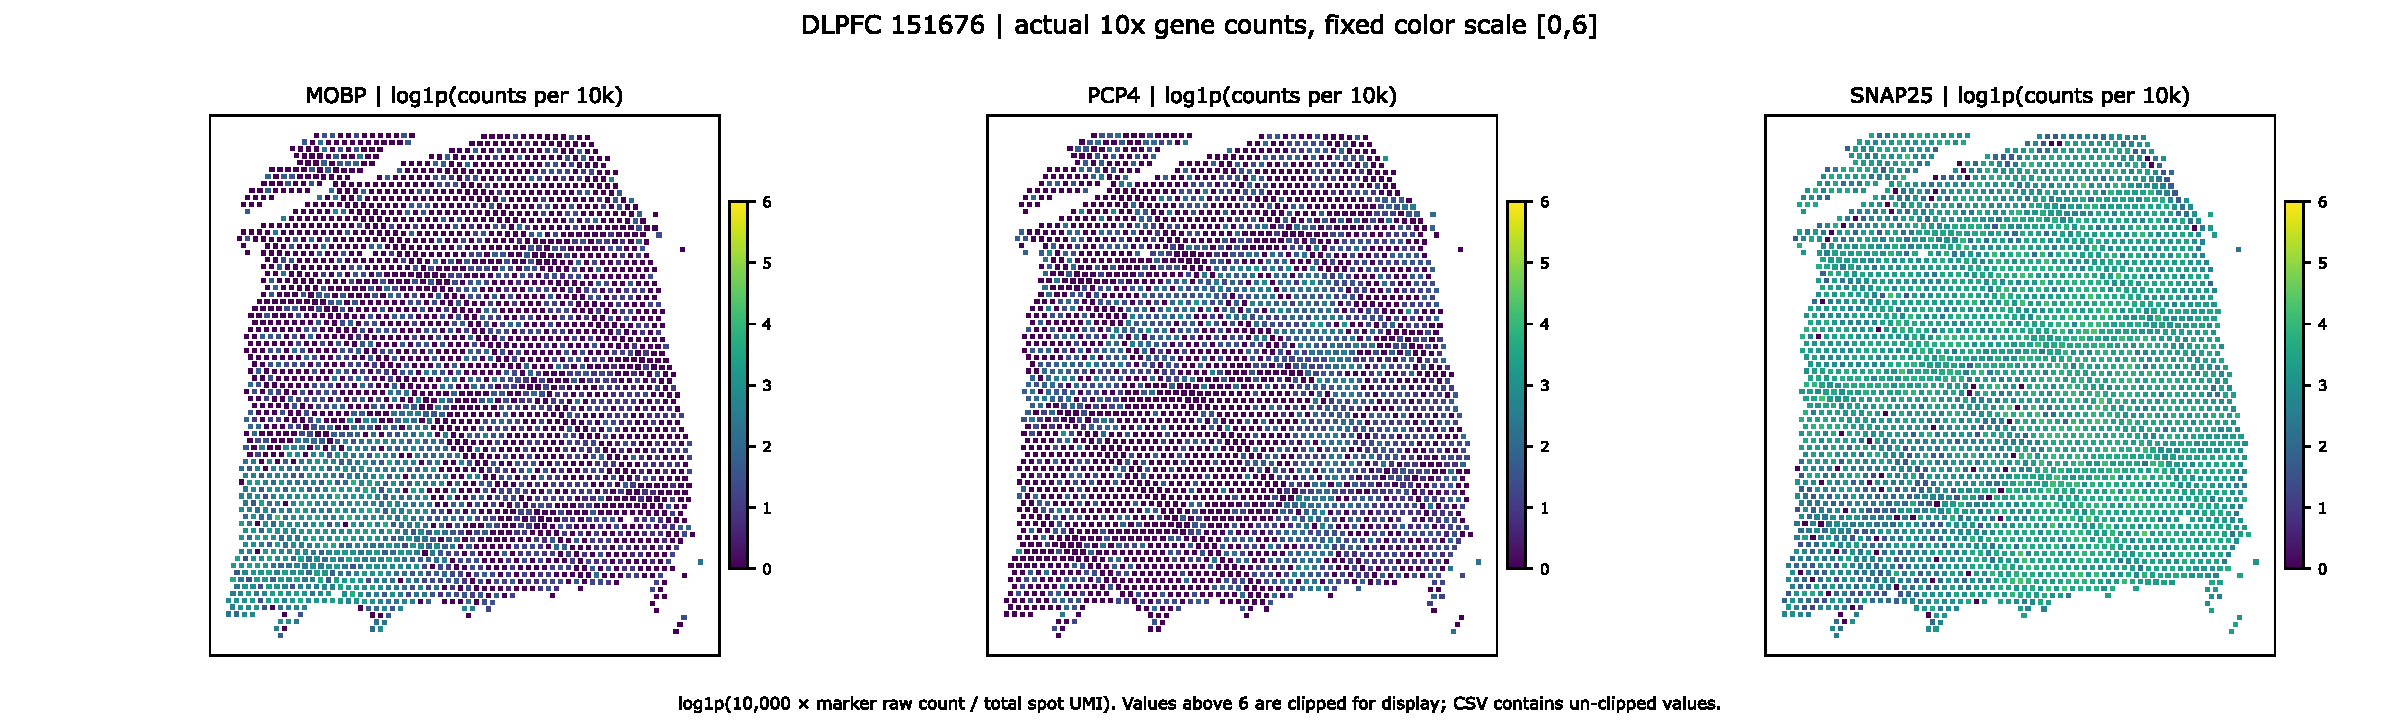
\includegraphics[width=0.97\linewidth,height=0.72\textheight,keepaspectratio]{E4_SOURCE_FIGURES_20261122_RELEASE/figures_pdf/151676/151676_MOBP_PCP4_SNAP25_expression.pdf}
\captionof{figure}{DLPFC切片151676：MOBP/PCP4/SNAP25表达三联图（原始E4图件转换的矢量PDF；聚类编号未根据参考标签重排）。}
\label{fig:cc-e4-app-151676-markers}
\end{minipage}\par\medskip
}{%
\par\noindent\emph{[编译提示：未找到该图件的PDF，请检查相对路径。]}\par
}
\IfFileExists{E4_SOURCE_FIGURES_20261122_RELEASE/figures_pdf/151676/151676_reference_A_B_confusion.pdf}{%
\par\noindent\begin{minipage}{\linewidth}
\centering
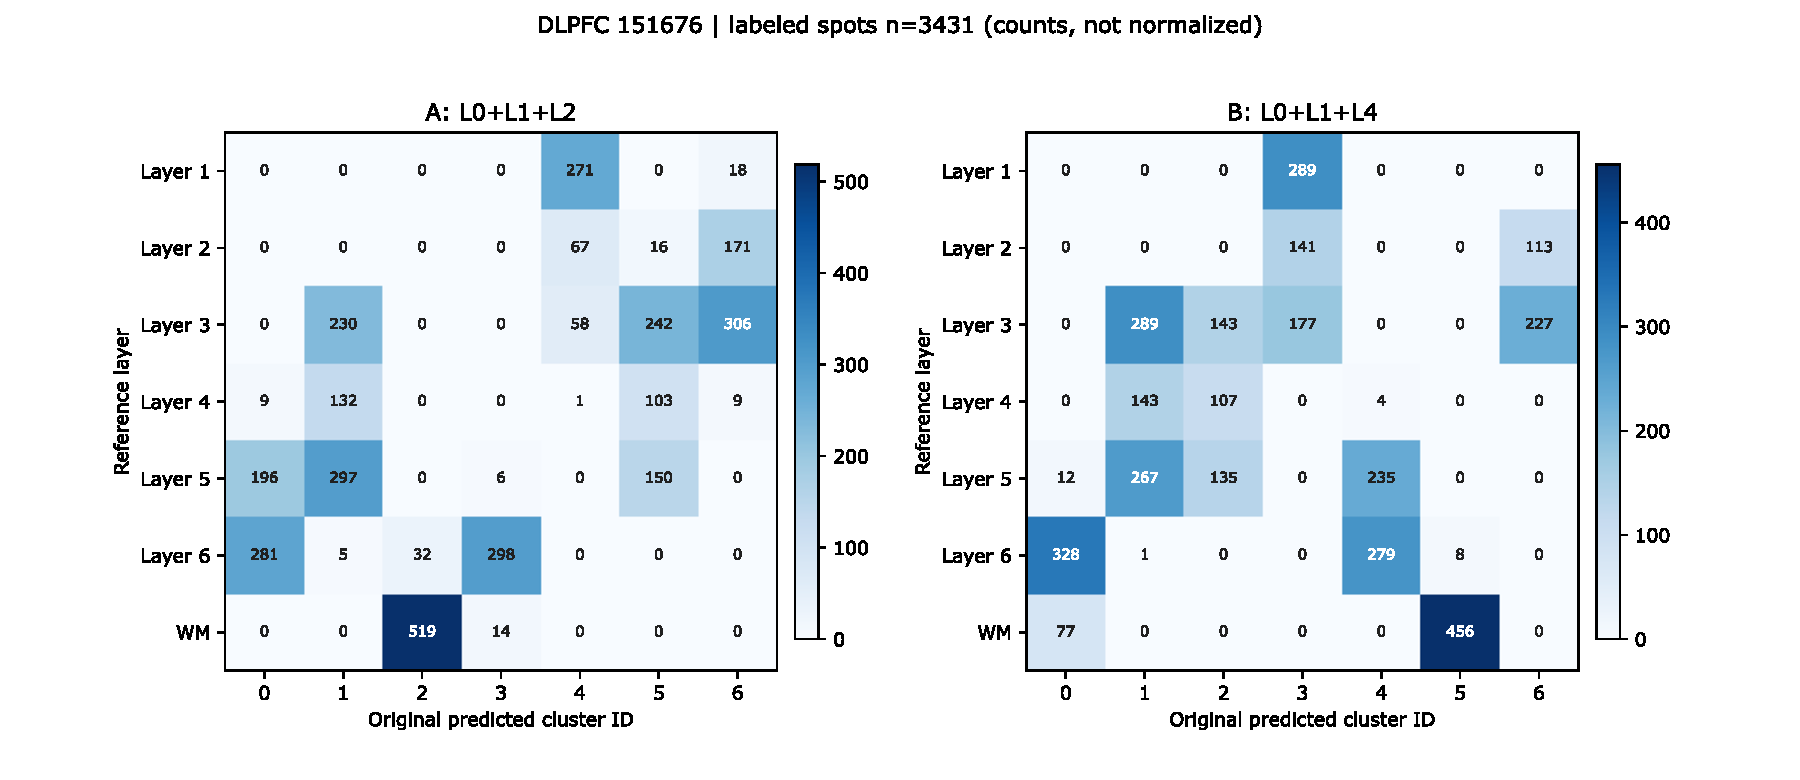
\includegraphics[width=0.97\linewidth,height=0.72\textheight,keepaspectratio]{E4_SOURCE_FIGURES_20261122_RELEASE/figures_pdf/151676/151676_reference_A_B_confusion.pdf}
\captionof{figure}{DLPFC切片151676：参考层与A/B簇交叉计数图（原始E4图件转换的矢量PDF；聚类编号未根据参考标签重排）。}
\label{fig:cc-e4-app-151676-confusion}
\end{minipage}\par\medskip
}{%
\par\noindent\emph{[编译提示：未找到该图件的PDF，请检查相对路径。]}\par
}
